\chapter{Huaraz, Cordillera Blanca et Trujillo}
\section*{13 juin 2015}
Huaraz est situé à environ 3000m d'altitude au coeur de la Cordillera Blanca, chaîne de montagnes avec plusieurs sommets à plus de 6000m dont le fameux Mont Huascaran. \newline
 \newline
\centerline{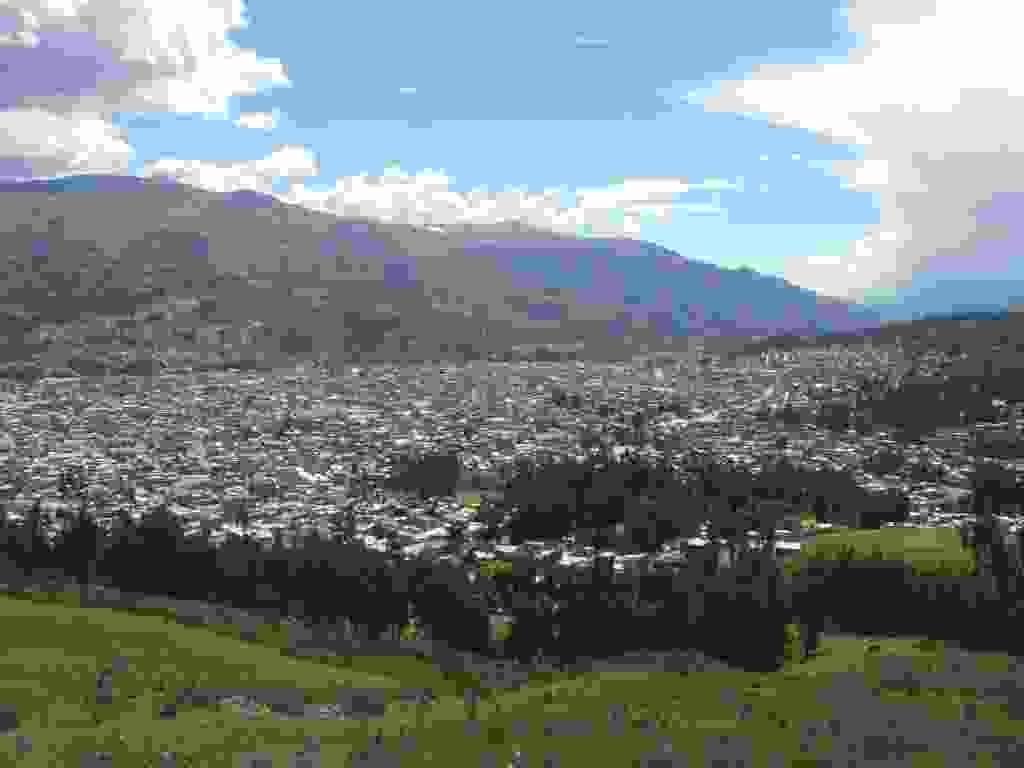
\includegraphics[height=90mm]{../wp-content/uploads/2015/06/P6034650-1024x768.jpg} } 
 \newline
 \newline
\centerline{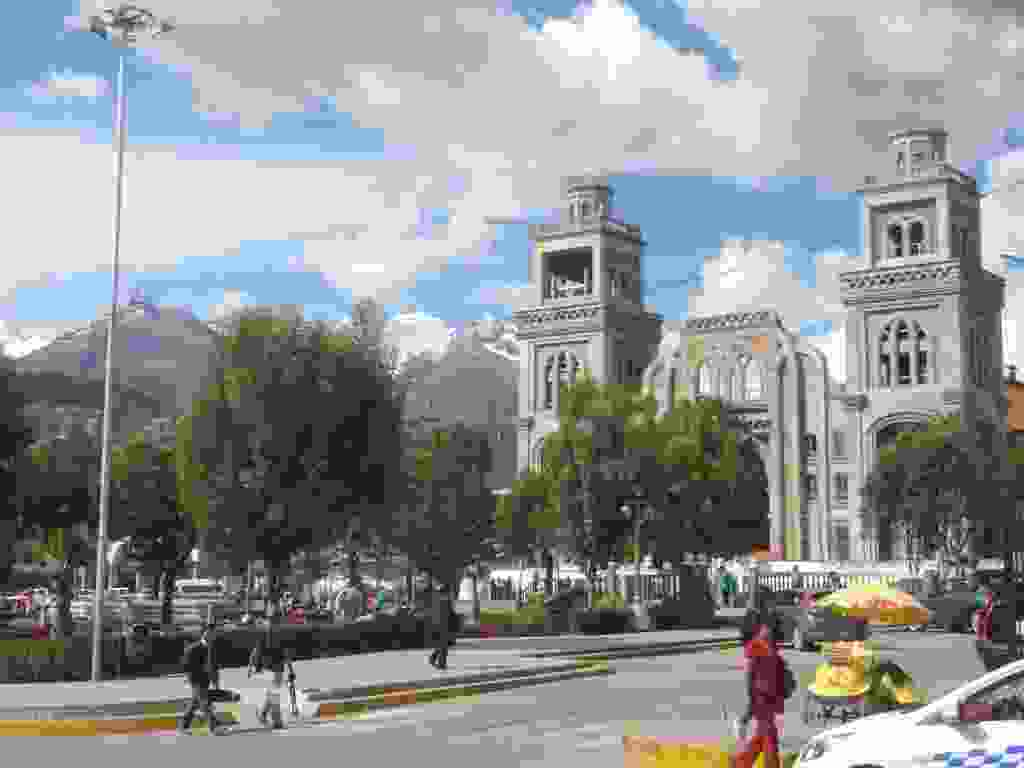
\includegraphics[height=90mm]{../wp-content/uploads/2015/06/P6034653-1024x768.jpg} } 
 \newline
 Marché d´Huaraz : \newline
 \newline
\centerline{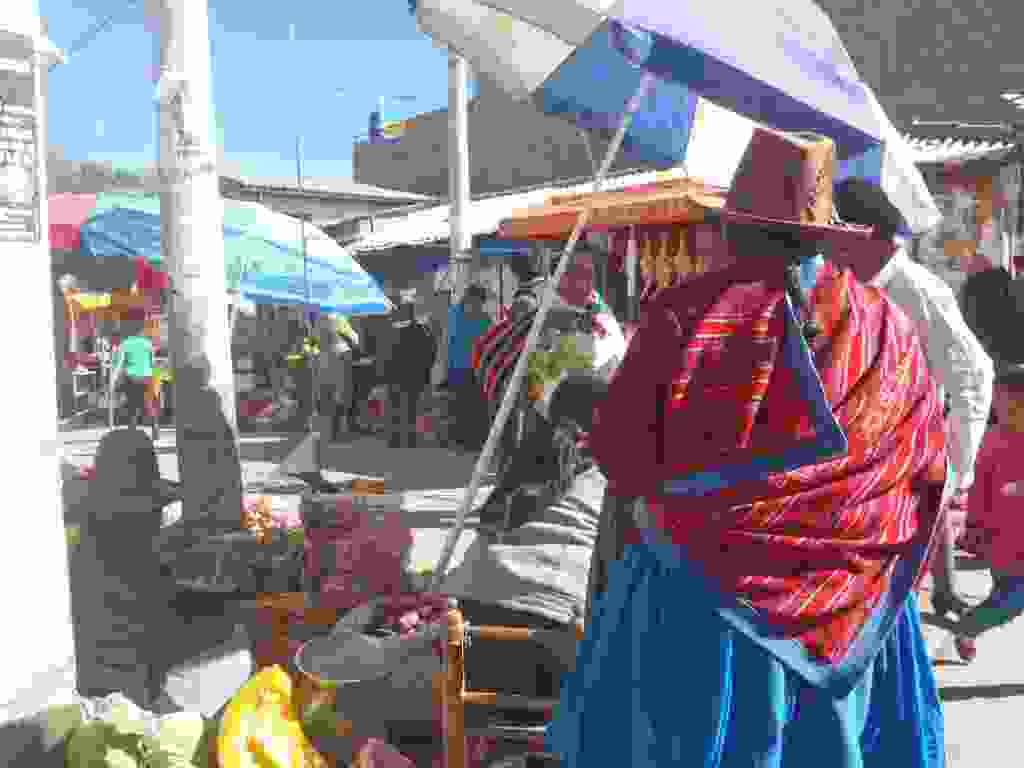
\includegraphics[height=90mm]{../wp-content/uploads/2015/06/P6034638-1024x768.jpg} } 
 \newline
 \newline
\centerline{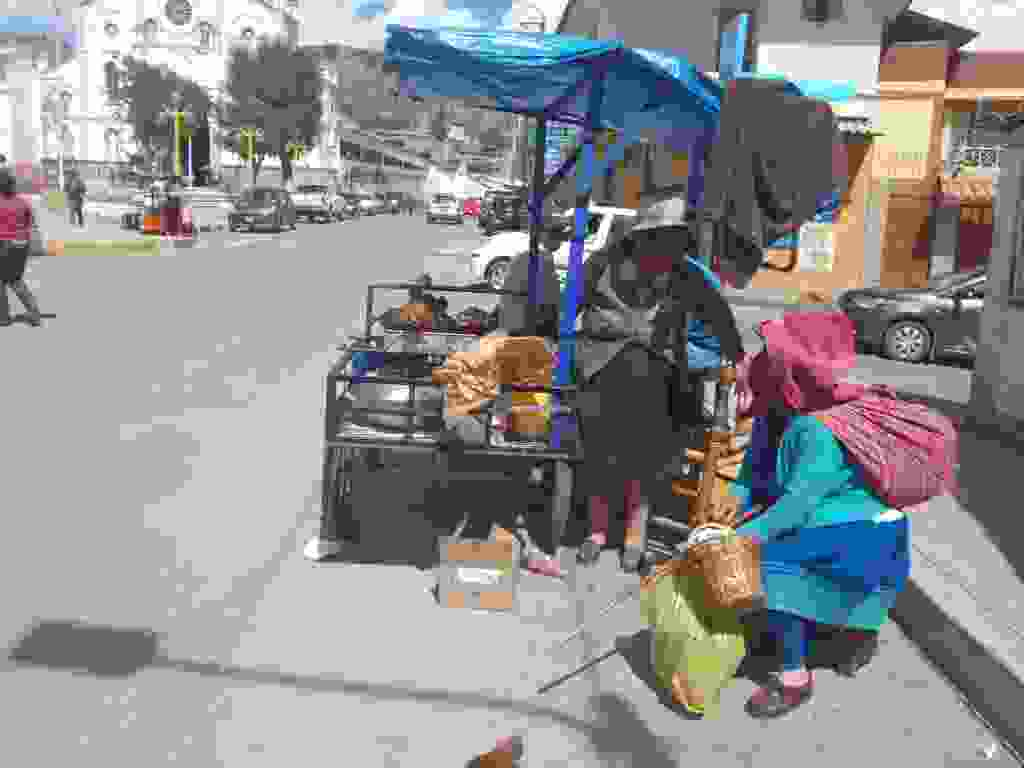
\includegraphics[height=90mm]{../wp-content/uploads/2015/06/P6034642-1024x768.jpg} } 
 \newline
 J'aurais bien tenté un sommet dans le parc national Huascaran mais le temps qui me reste jusqu'en Equateur et le prix des ascensions m'ont dissuadés. \newline
 À la place j'ai fait 2 randonnées à la journée : \newline
 D'abord juste au dessus d´Huaraz pour aller voir la Laguna Churup. \newline
 \newline
\centerline{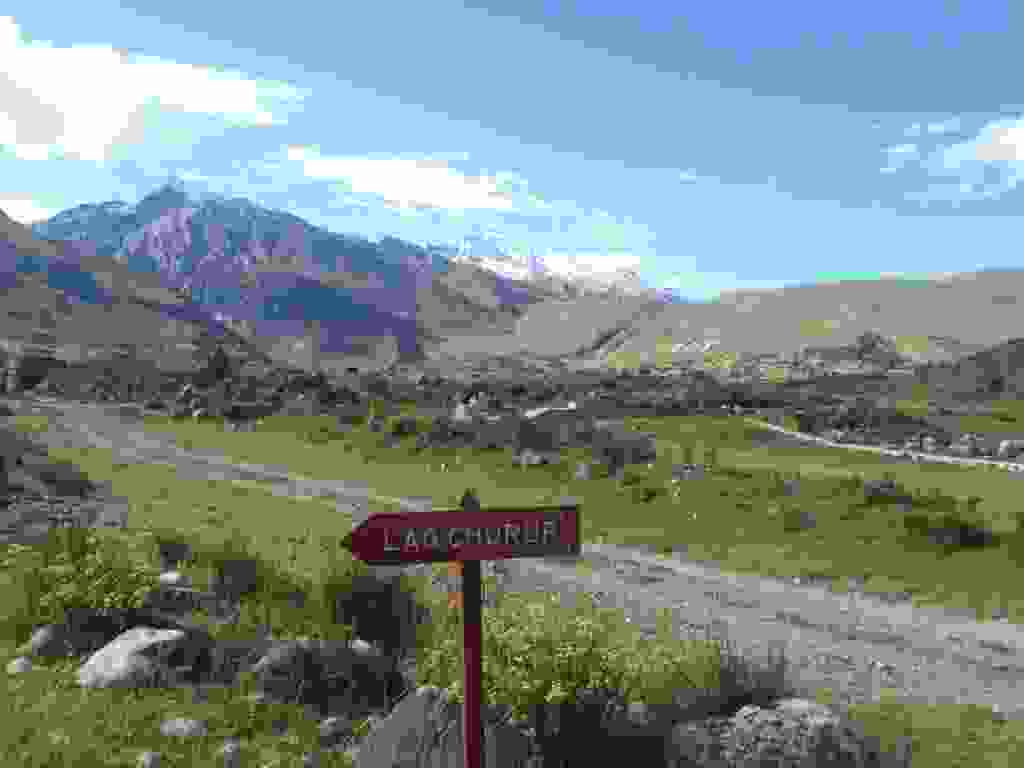
\includegraphics[height=90mm]{../wp-content/uploads/2015/06/P6044656-1024x768.jpg} } 
 \newline
 \newline
\centerline{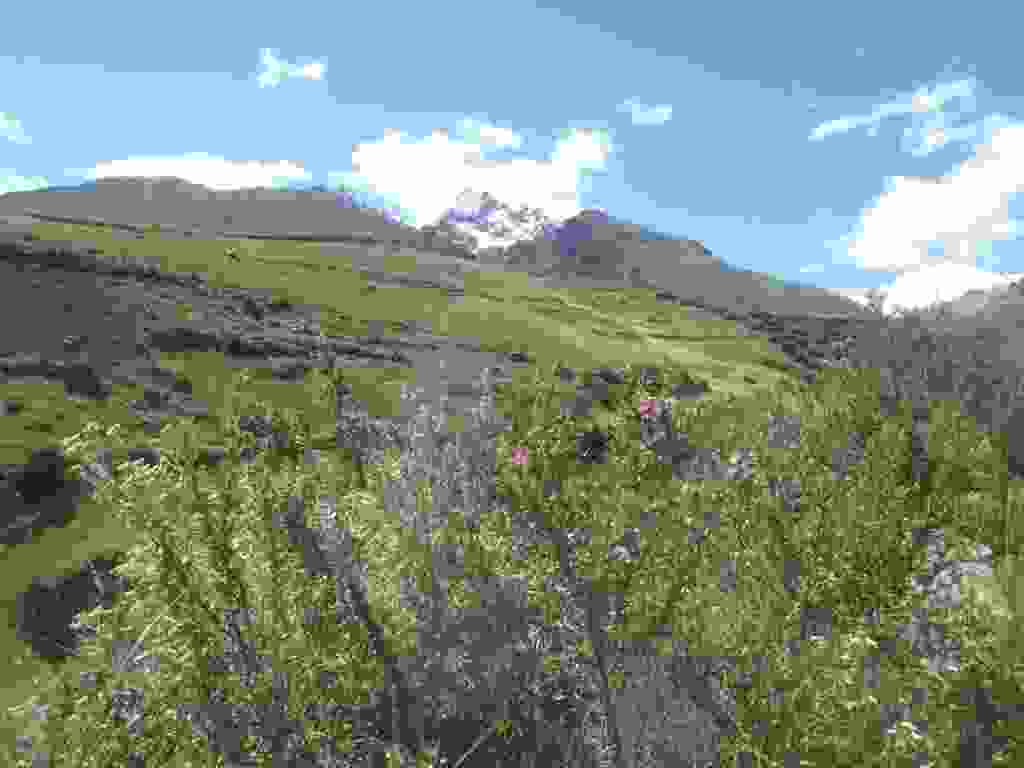
\includegraphics[height=90mm]{../wp-content/uploads/2015/06/P6044679-1024x768.jpg} } 
 \newline
 \newline
\centerline{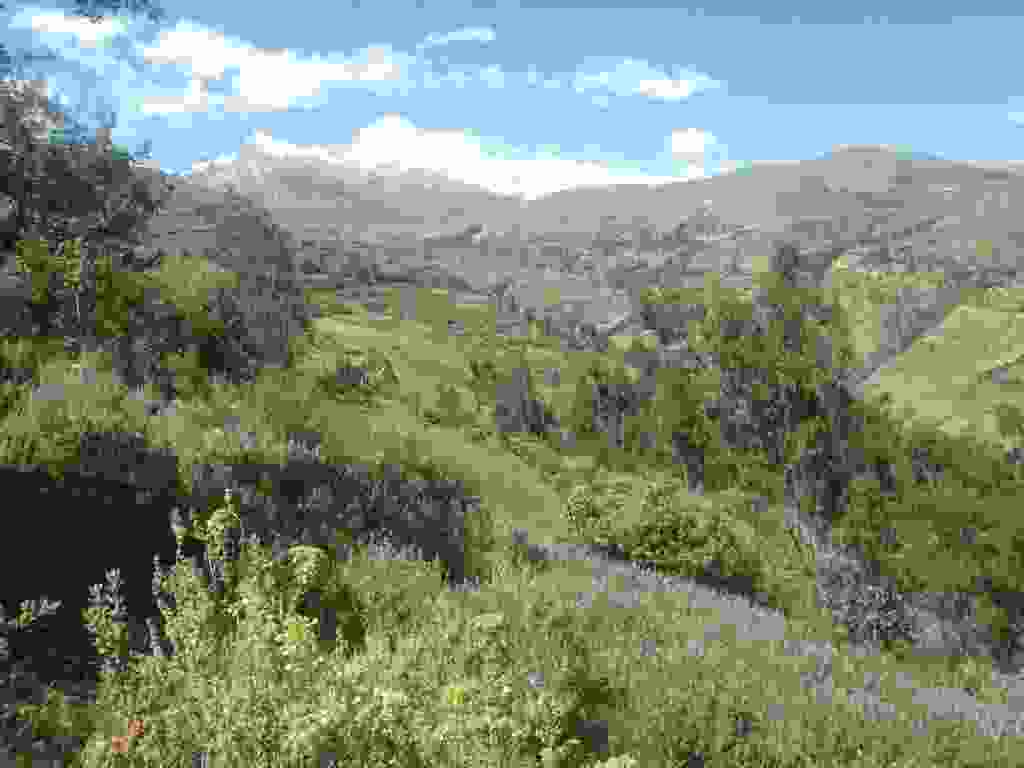
\includegraphics[height=90mm]{../wp-content/uploads/2015/06/P6044681-1024x768.jpg} } 
 \newline
 \newline
\centerline{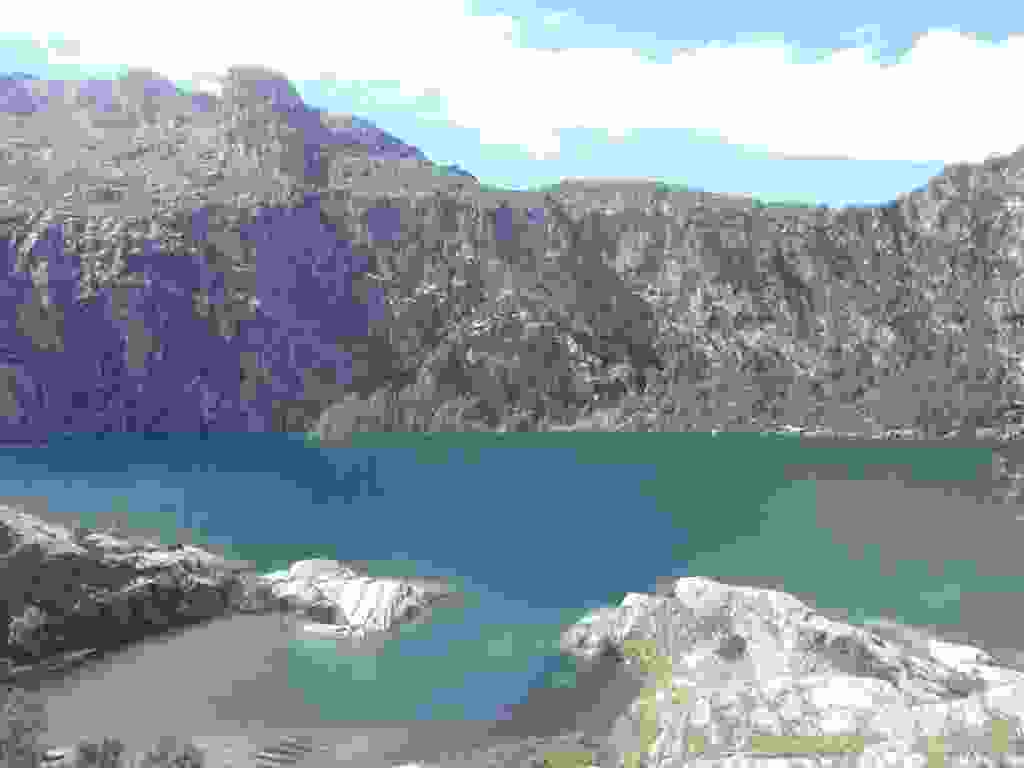
\includegraphics[height=90mm]{../wp-content/uploads/2015/06/P6044670-1024x768.jpg} } 
 \newline
 \newline
\centerline{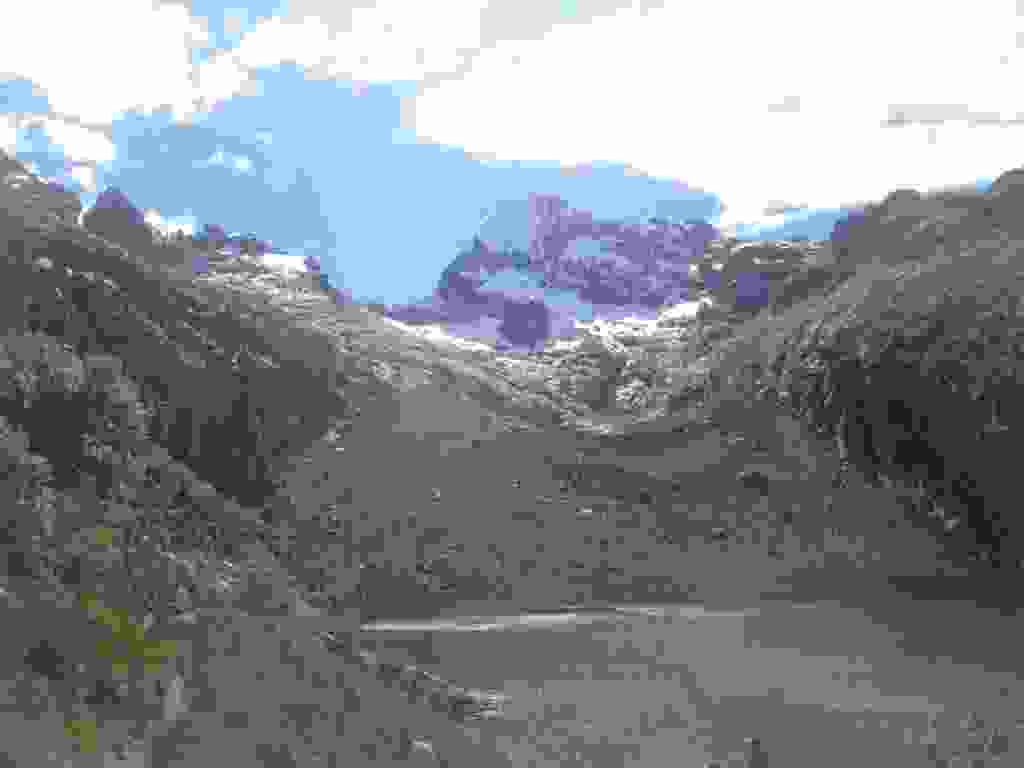
\includegraphics[height=90mm]{../wp-content/uploads/2015/06/P6044674-1024x768.jpg} } 
 \newline
 Puis une journée de vélo plus loin, la Laguna 69. J'ai fait la rando avec Elise et Laurent, cyclistes rencontrés le matin. \newline
 \newline
\centerline{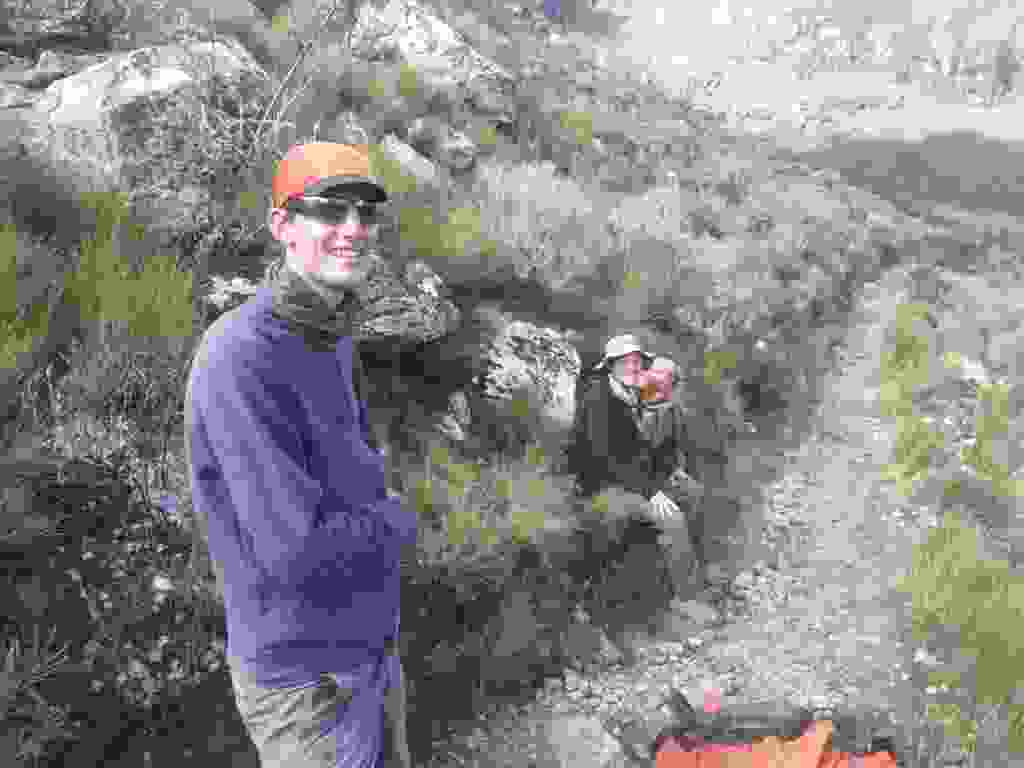
\includegraphics[height=90mm]{../wp-content/uploads/2015/06/P6064713-1024x768.jpg} } 
 \newline
 \newline
\centerline{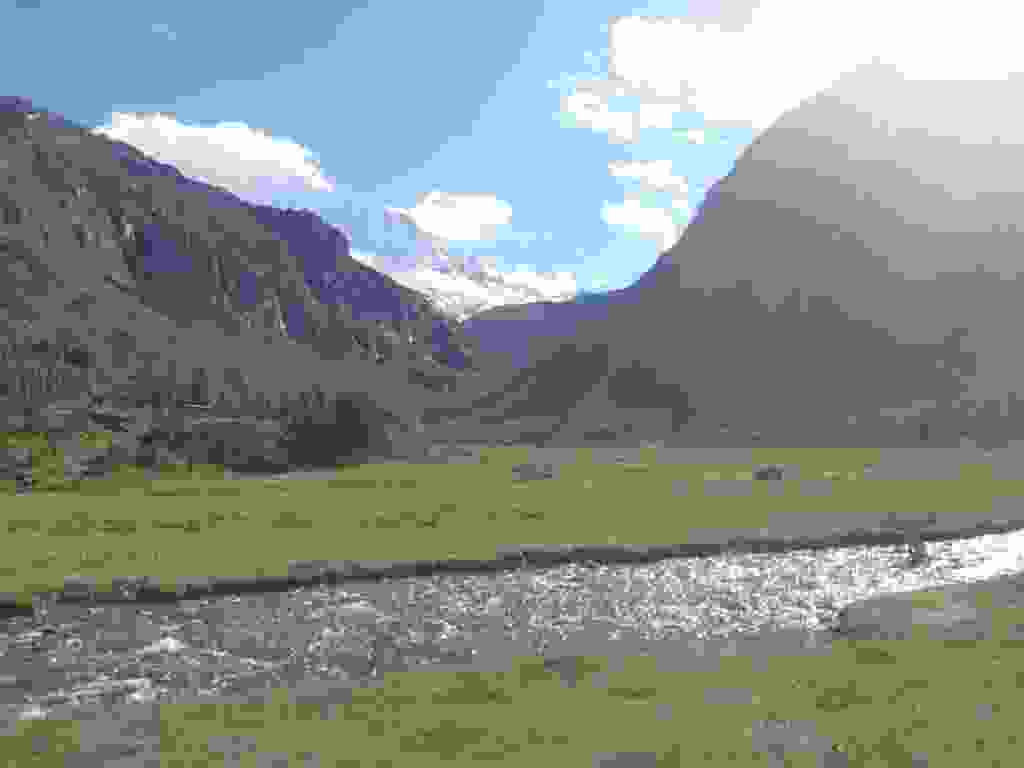
\includegraphics[height=90mm]{../wp-content/uploads/2015/06/P6064706-1024x768.jpg} } 
 \newline
 \newline
\centerline{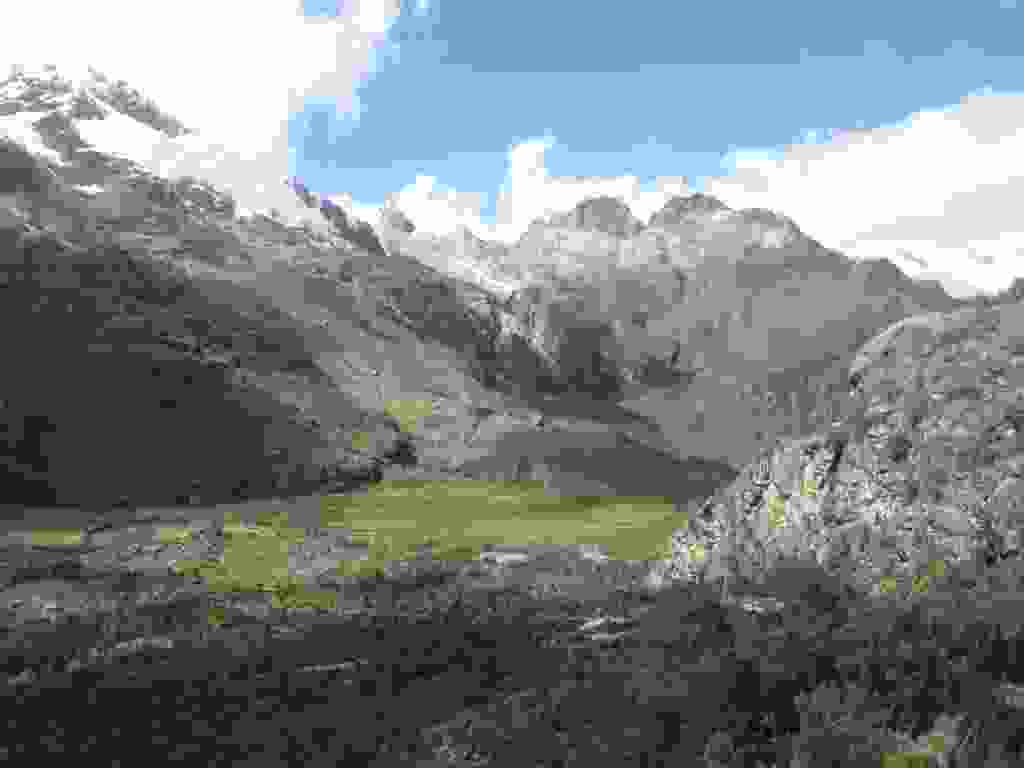
\includegraphics[height=90mm]{../wp-content/uploads/2015/06/P6064719-1024x768.jpg} } 
 \newline
 \newline
\centerline{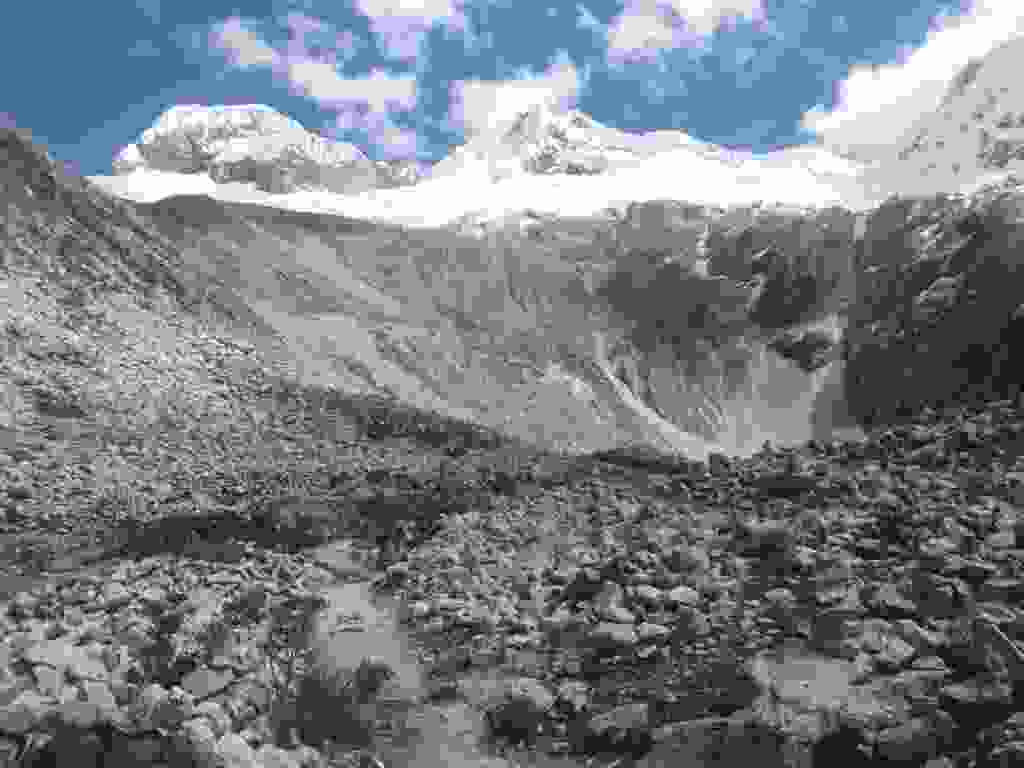
\includegraphics[height=90mm]{../wp-content/uploads/2015/06/P6064720-1024x768.jpg} } 
 \newline
 \newline
\centerline{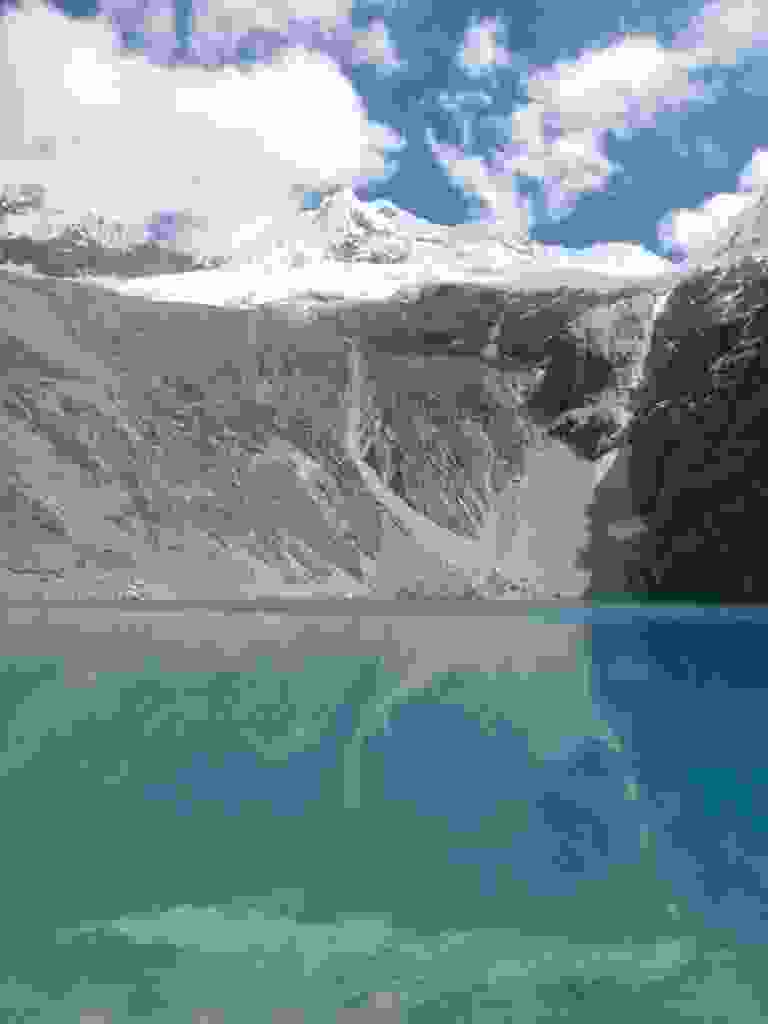
\includegraphics[height=90mm]{../wp-content/uploads/2015/06/P6064726-768x1024.jpg} } 
 \newline
 \newline
\centerline{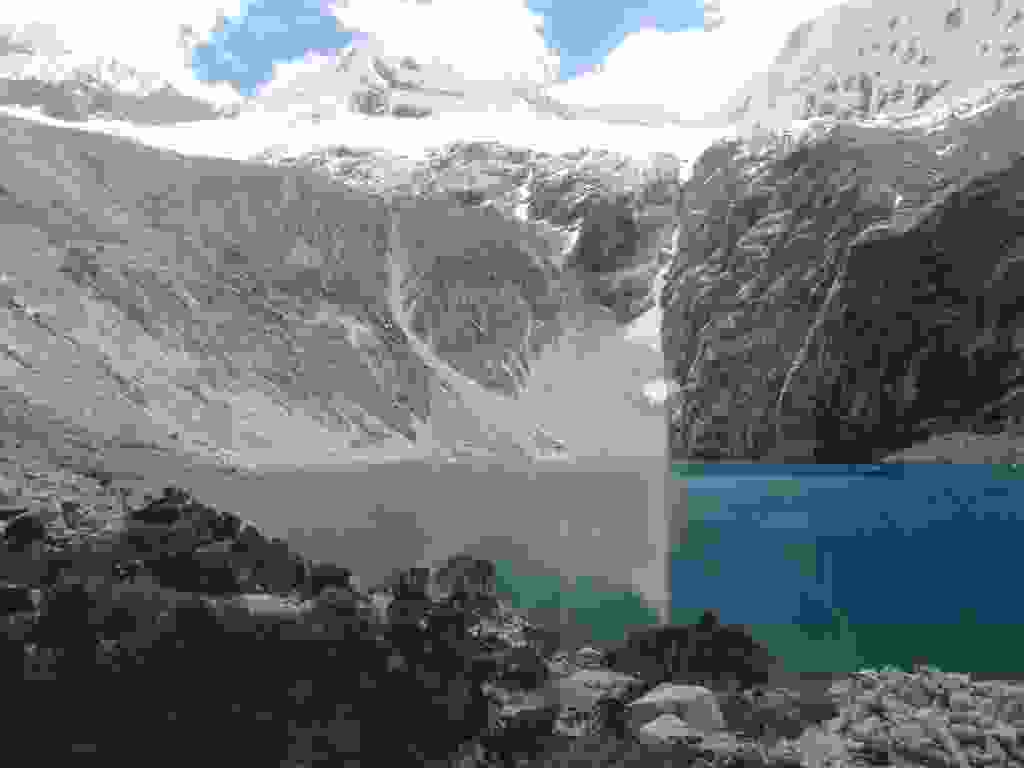
\includegraphics[height=90mm]{../wp-content/uploads/2015/06/P6064733-1024x768.jpg} } 
 \newline
 \newline
\centerline{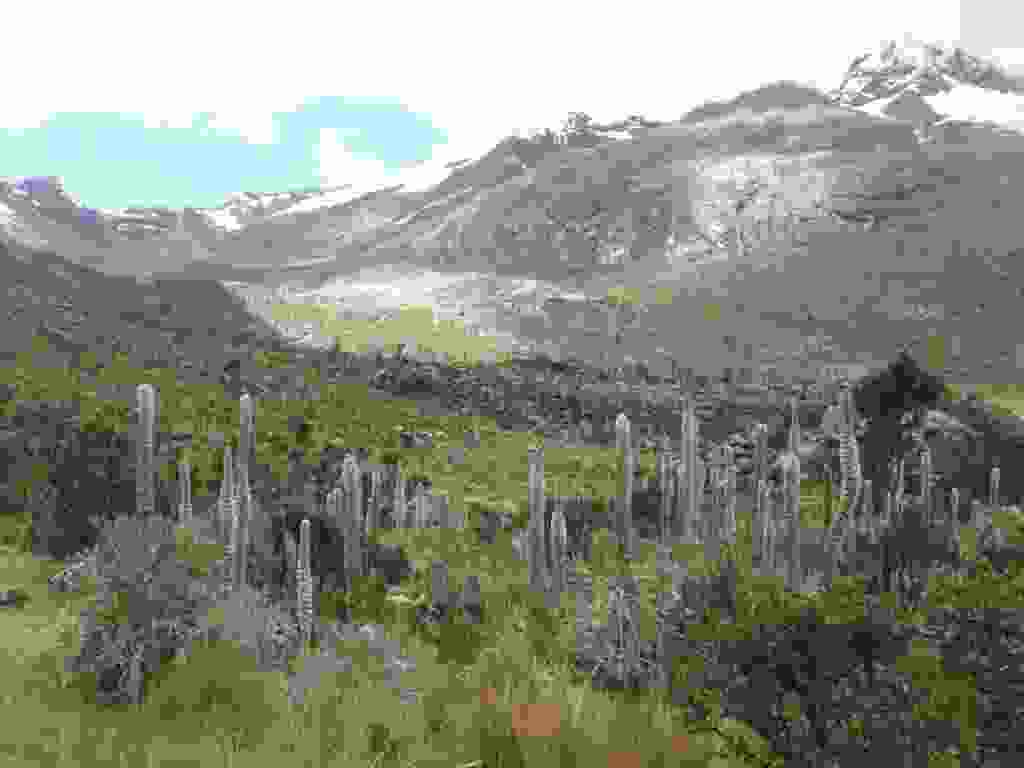
\includegraphics[height=90mm]{../wp-content/uploads/2015/06/P6064739-1024x768.jpg} } 
 \newline
 \newline
\centerline{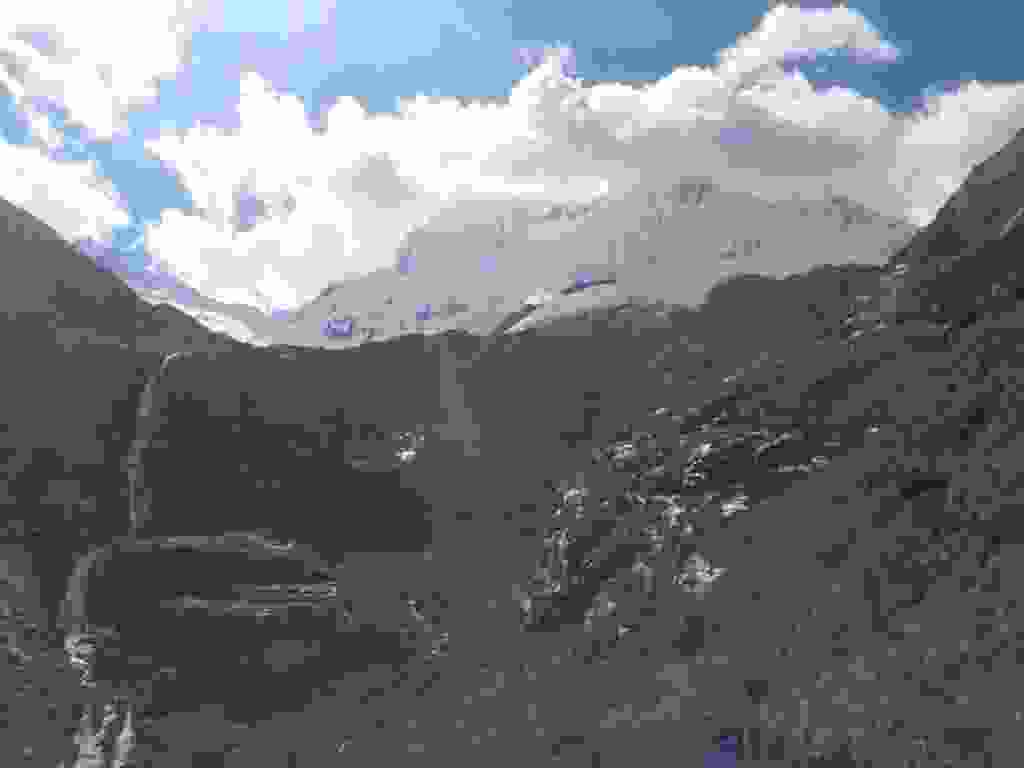
\includegraphics[height=90mm]{../wp-content/uploads/2015/06/P6064743-1024x768.jpg} } 
 \newline
 \newline
\centerline{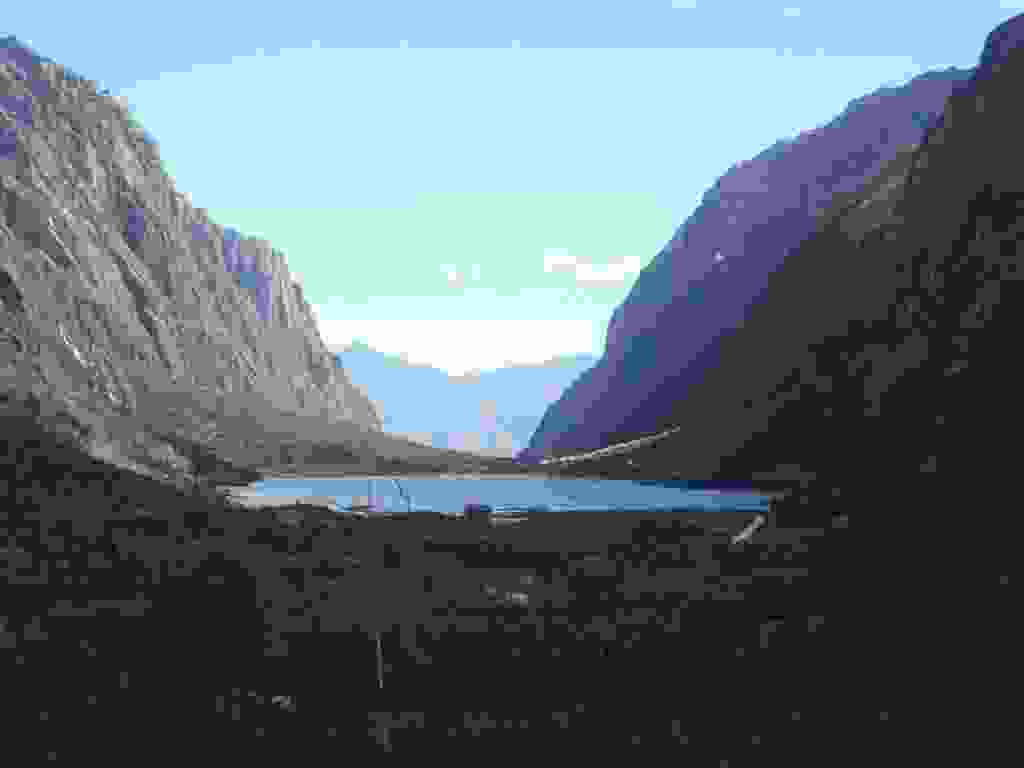
\includegraphics[height=90mm]{../wp-content/uploads/2015/06/P6064745-1024x768.jpg} } 
 \newline
 J'ai ensuite repris le vélo sur la route qui longe la Cordillera Blanca. J´y ai croisé quelques voyageurs à vélo et à moto. \newline
 \newline
\centerline{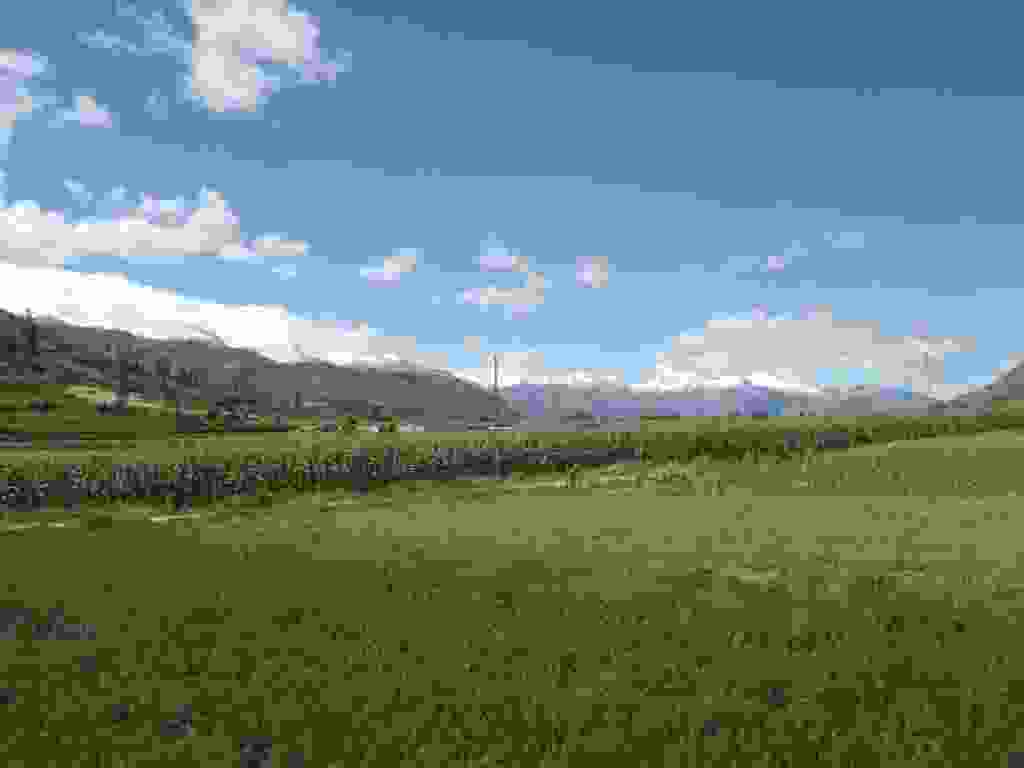
\includegraphics[height=90mm]{../wp-content/uploads/2015/06/P6054697-1024x768.jpg} } 
 \newline
 \newline
\centerline{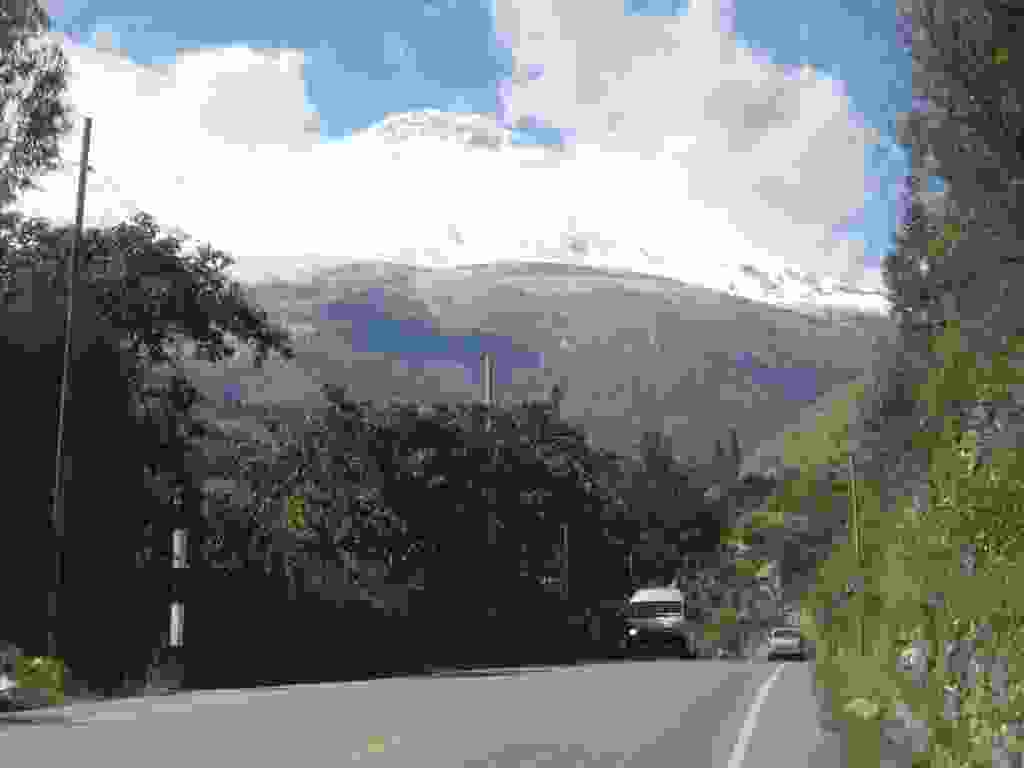
\includegraphics[height=90mm]{../wp-content/uploads/2015/06/P6054699-1024x768.jpg} } 
 \newline
 \newline
\centerline{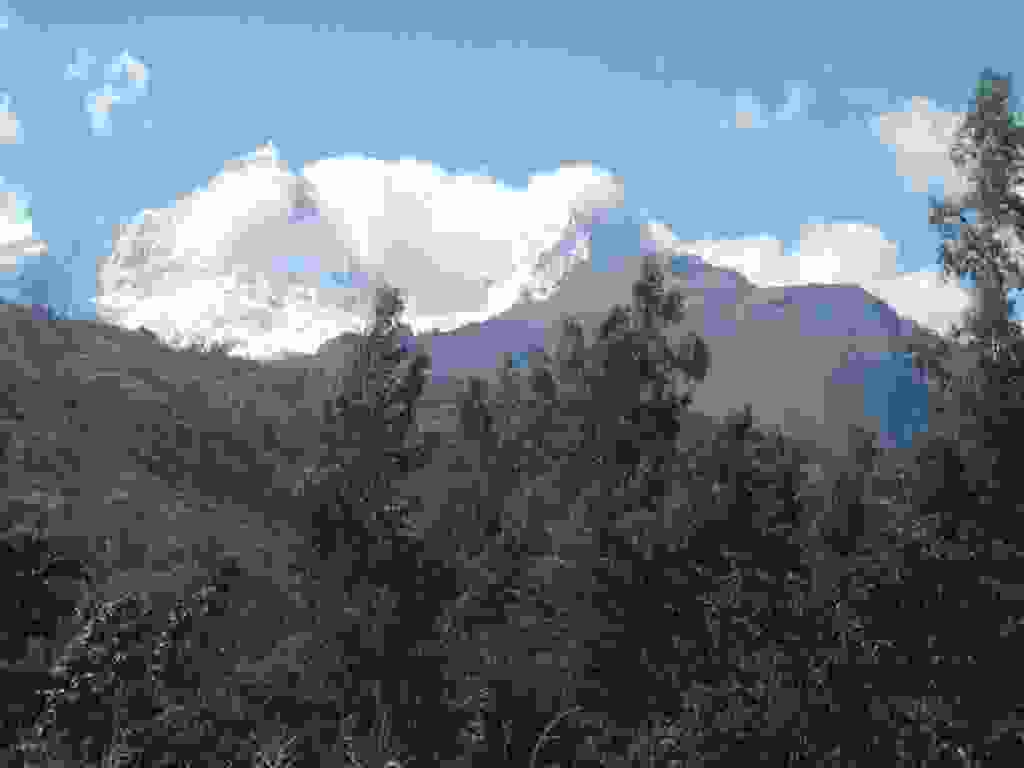
\includegraphics[height=90mm]{../wp-content/uploads/2015/06/P6054701-1024x768.jpg} } 
 \newline
 Ensuite descente du canyon del Pato et ses dizaines de tunnels. \newline
 \newline
\centerline{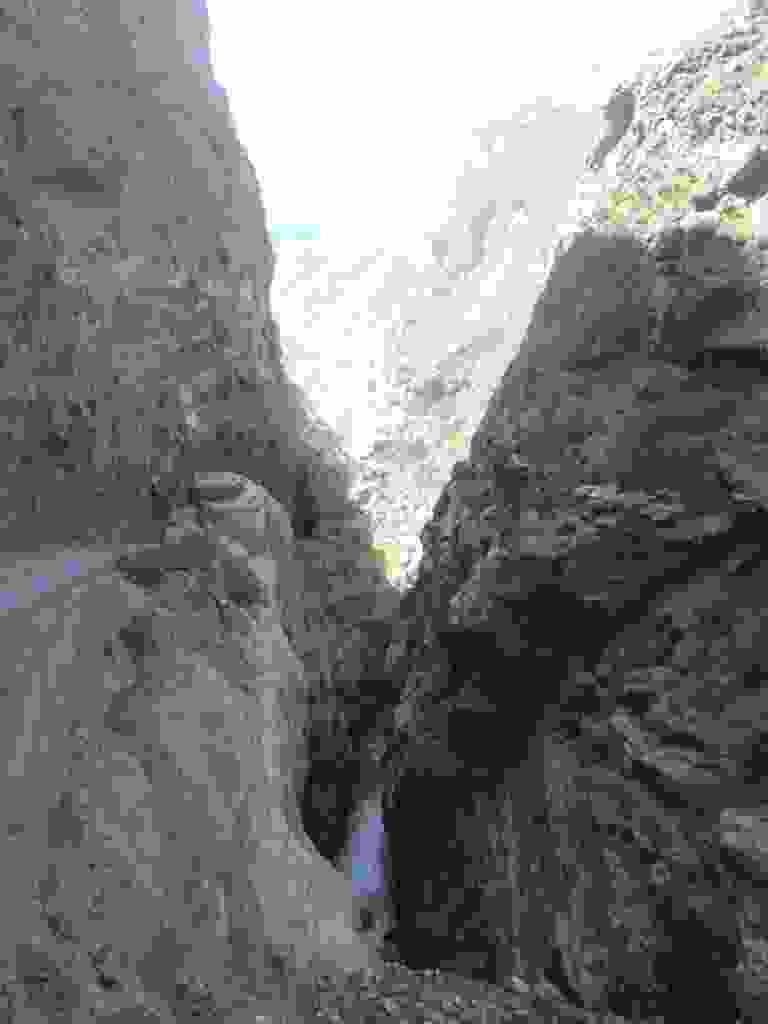
\includegraphics[height=90mm]{../wp-content/uploads/2015/06/P6074761-768x1024.jpg} } 
 \newline
 \newline
\centerline{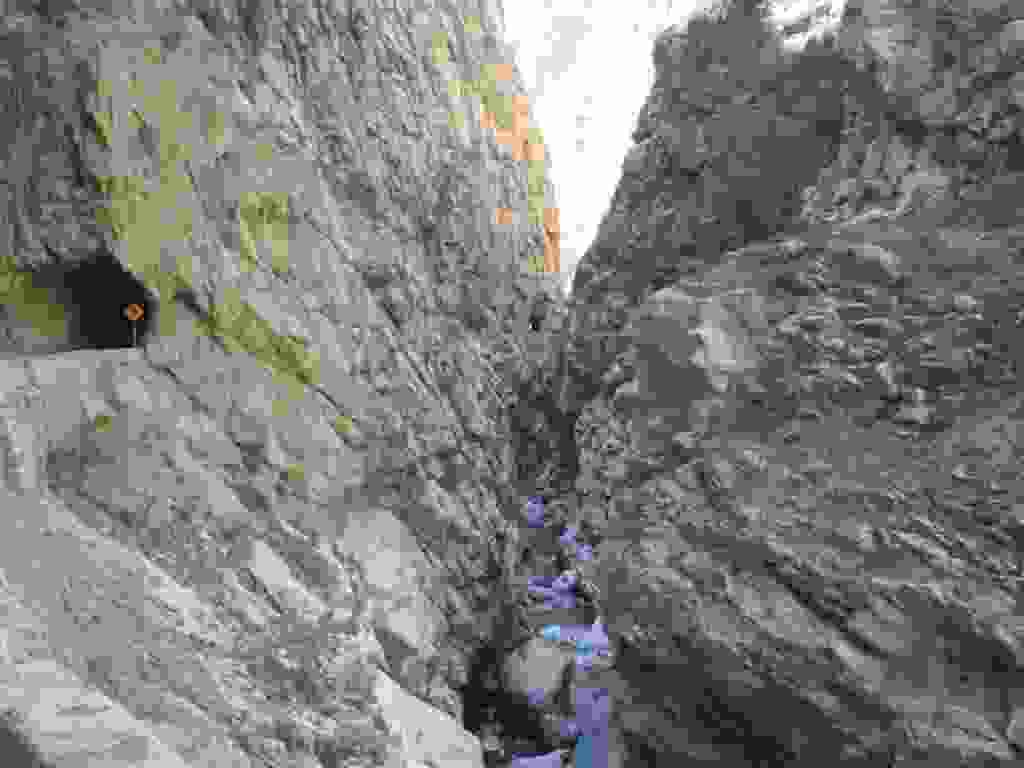
\includegraphics[height=90mm]{../wp-content/uploads/2015/06/P6074764-1024x768.jpg} } 
 \newline
 \newline
\centerline{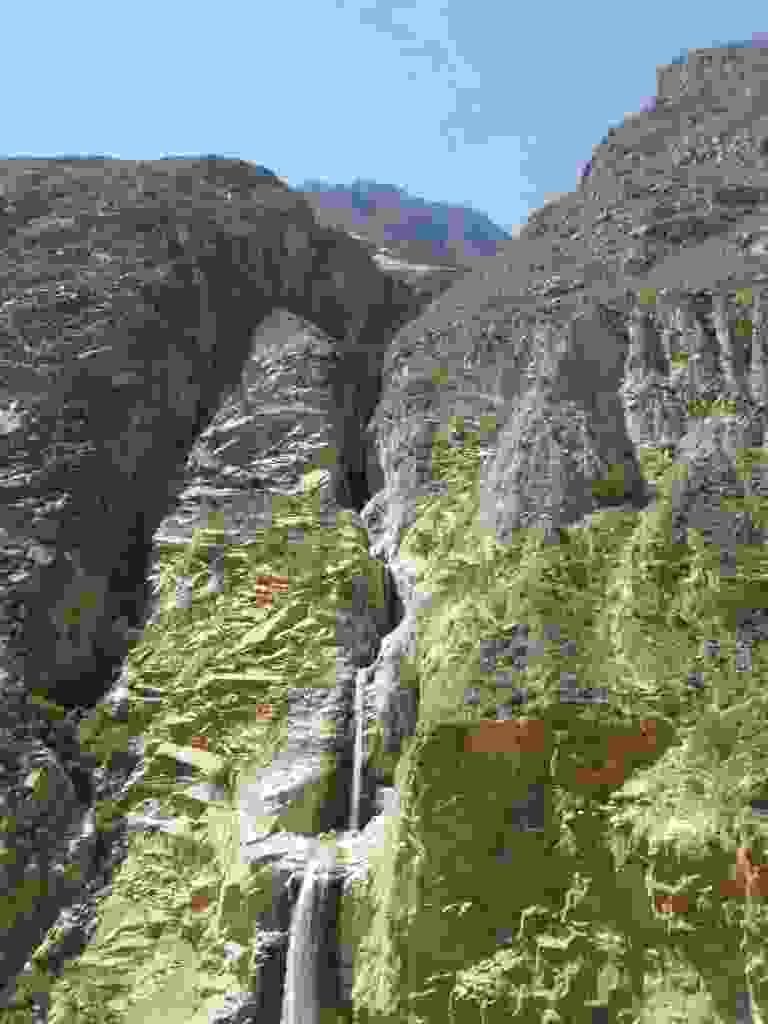
\includegraphics[height=90mm]{../wp-content/uploads/2015/06/P6074766-768x1024.jpg} } 
 \newline
 \newline
\centerline{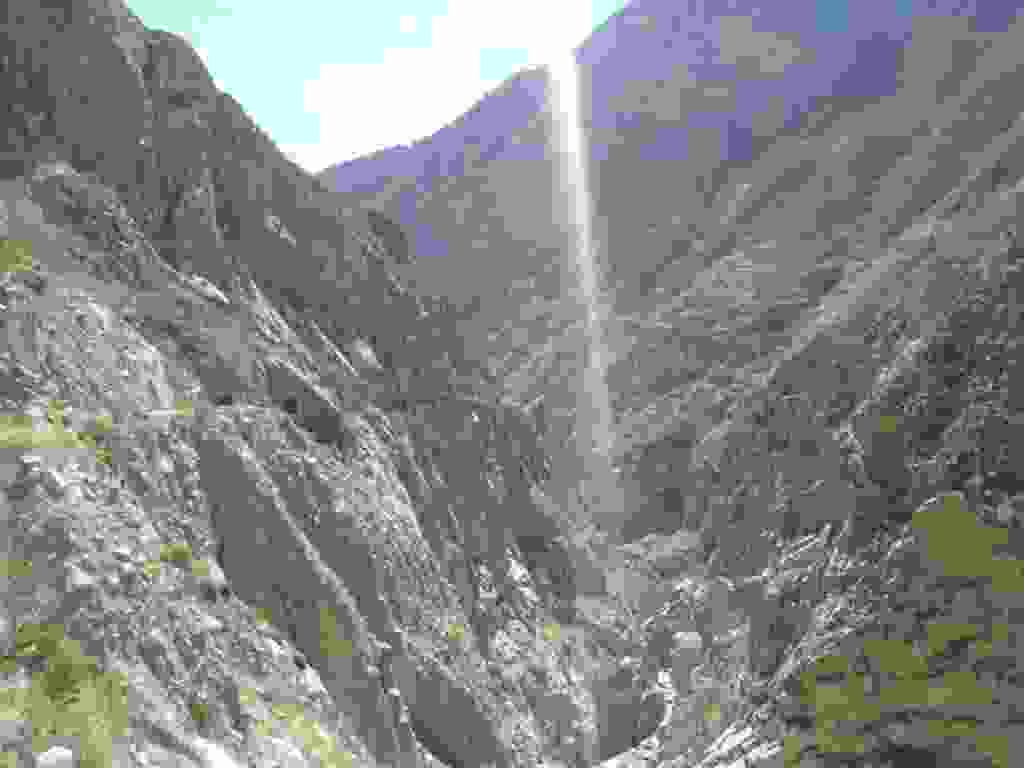
\includegraphics[height=90mm]{../wp-content/uploads/2015/06/P6074767-1024x768.jpg} } 
 \newline
 Puis je retrouve une piste non asphaltée, ça faisait un moment. \newline
 \newline
\centerline{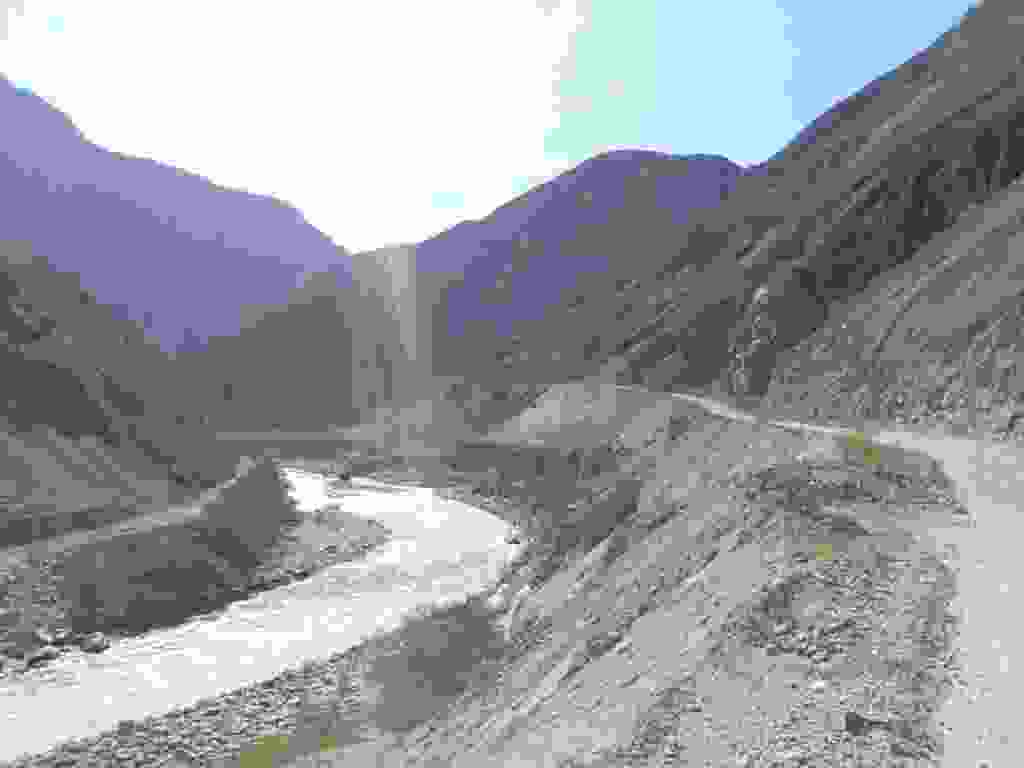
\includegraphics[height=90mm]{../wp-content/uploads/2015/06/P6074770-1024x768.jpg} } 
 \newline
 \newline
\centerline{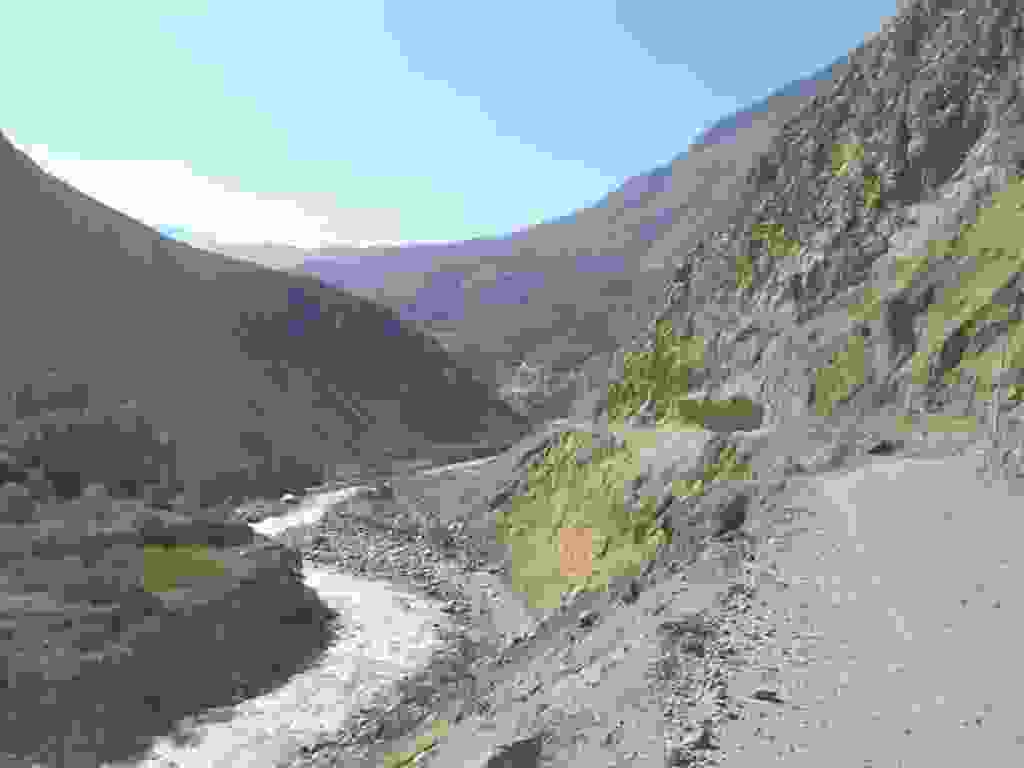
\includegraphics[height=90mm]{../wp-content/uploads/2015/06/P6074772-1024x768.jpg} } 
 \newline
 \newline
\centerline{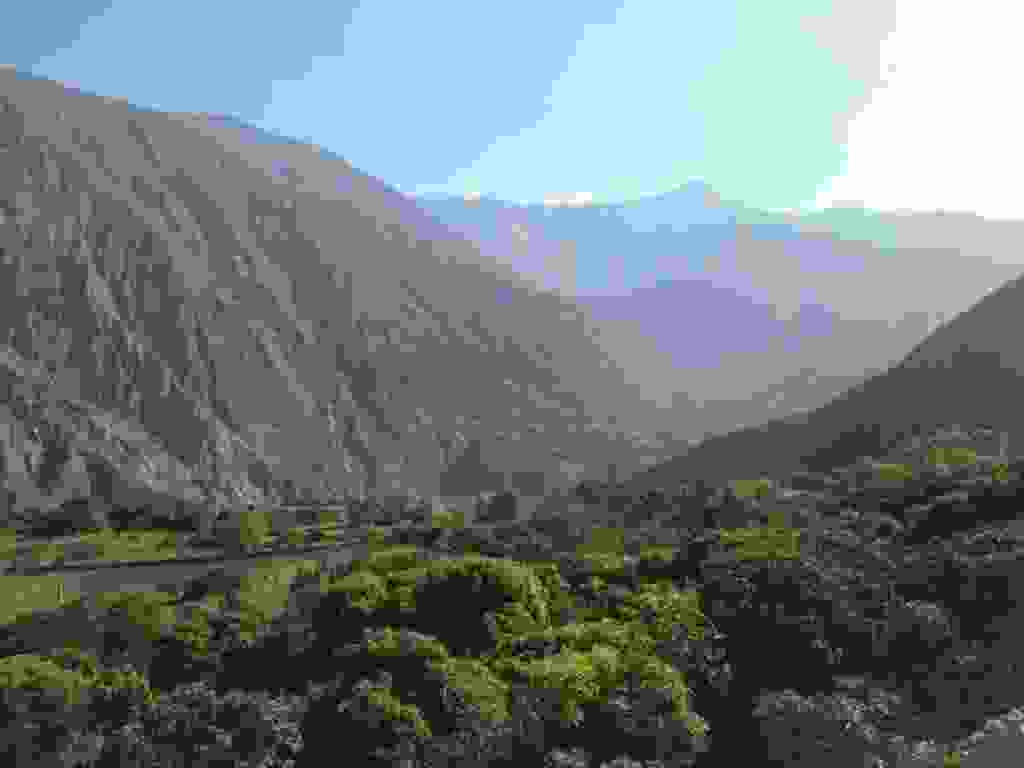
\includegraphics[height=90mm]{../wp-content/uploads/2015/06/P6074775-1024x768.jpg} } 
 \newline
 Encore une portion bien encaissée. \newline
 \newline
\centerline{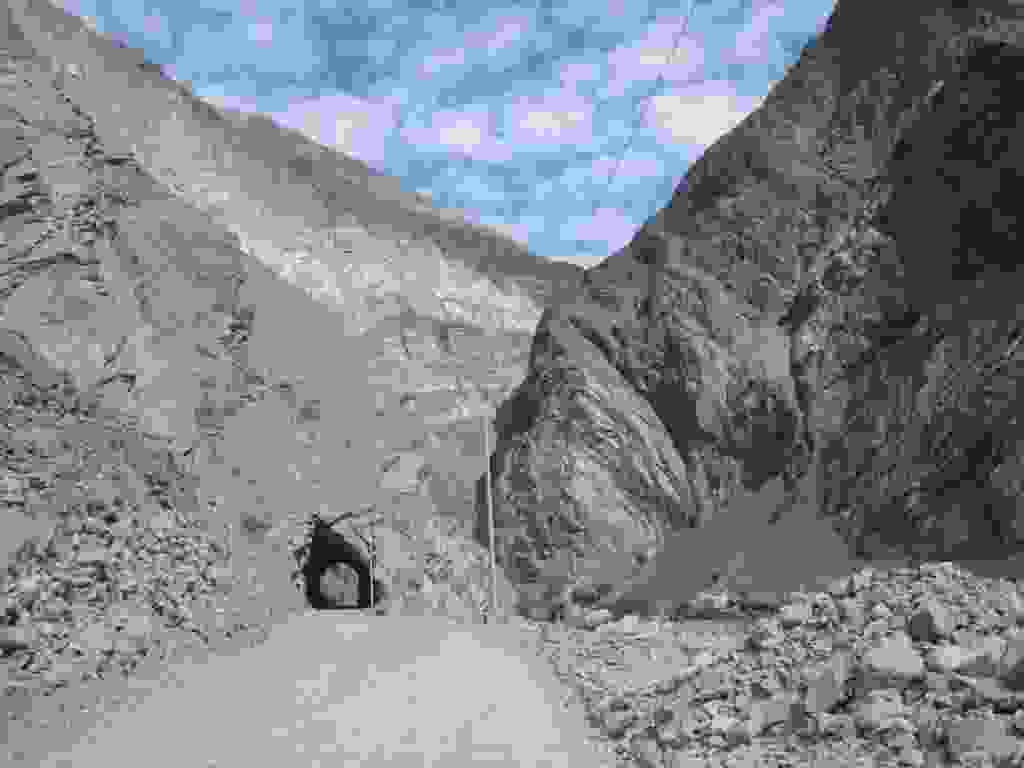
\includegraphics[height=90mm]{../wp-content/uploads/2015/06/P6084784-1024x768.jpg} } 
 \newline
 \newline
\centerline{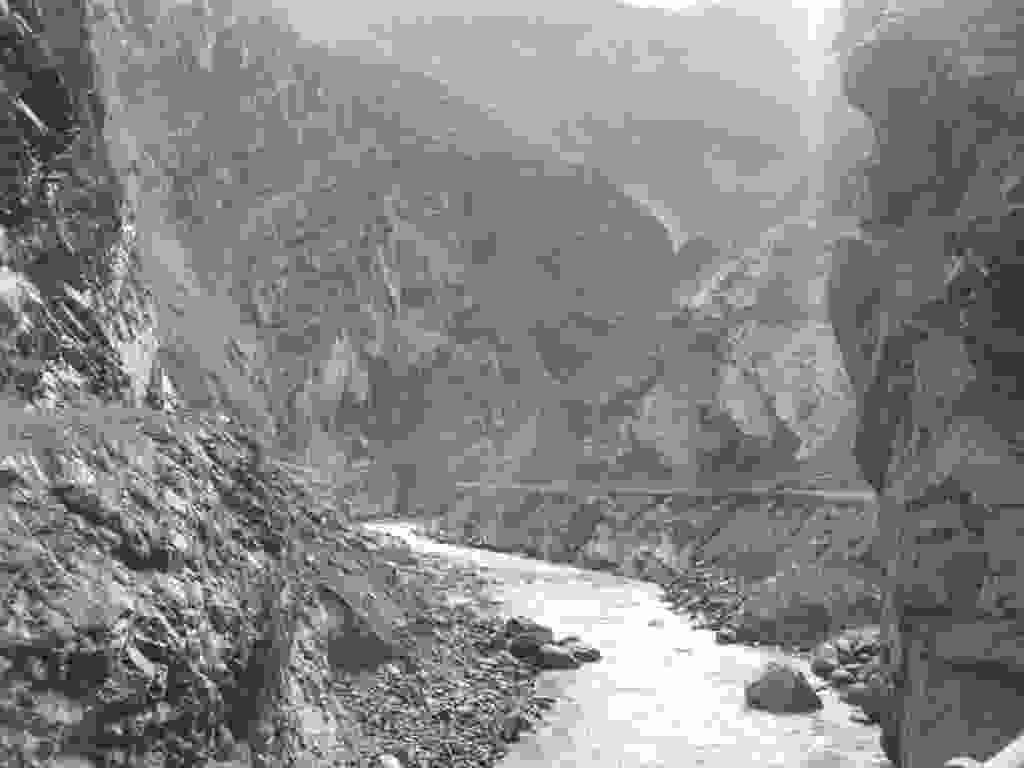
\includegraphics[height=90mm]{../wp-content/uploads/2015/06/P6084786-1024x768.jpg} } 
 \newline
 Je traverse de rares villages qui paraissent quasiment abandonnés. Peu de possibilités de ravitaillement sur cette route, j´étais content d´avoir le filtre pour prendre de l´eau dans la riviere. \newline
 \newline
\centerline{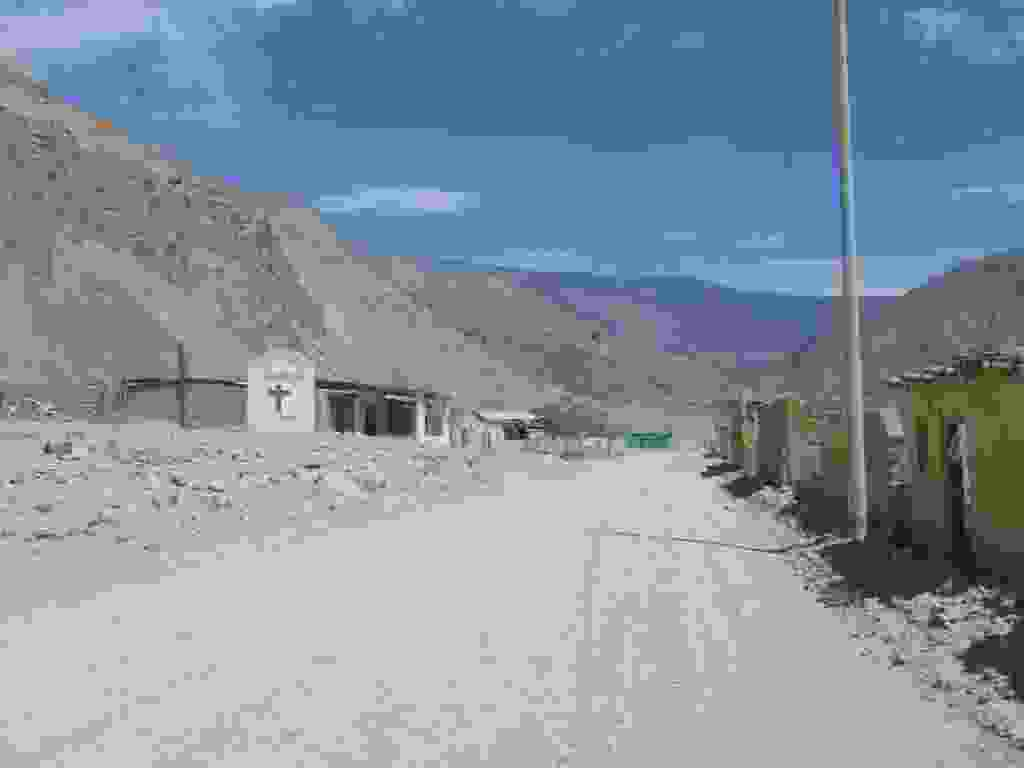
\includegraphics[height=90mm]{../wp-content/uploads/2015/06/P6084790-1024x768.jpg} } 
 \newline
 \newline
\centerline{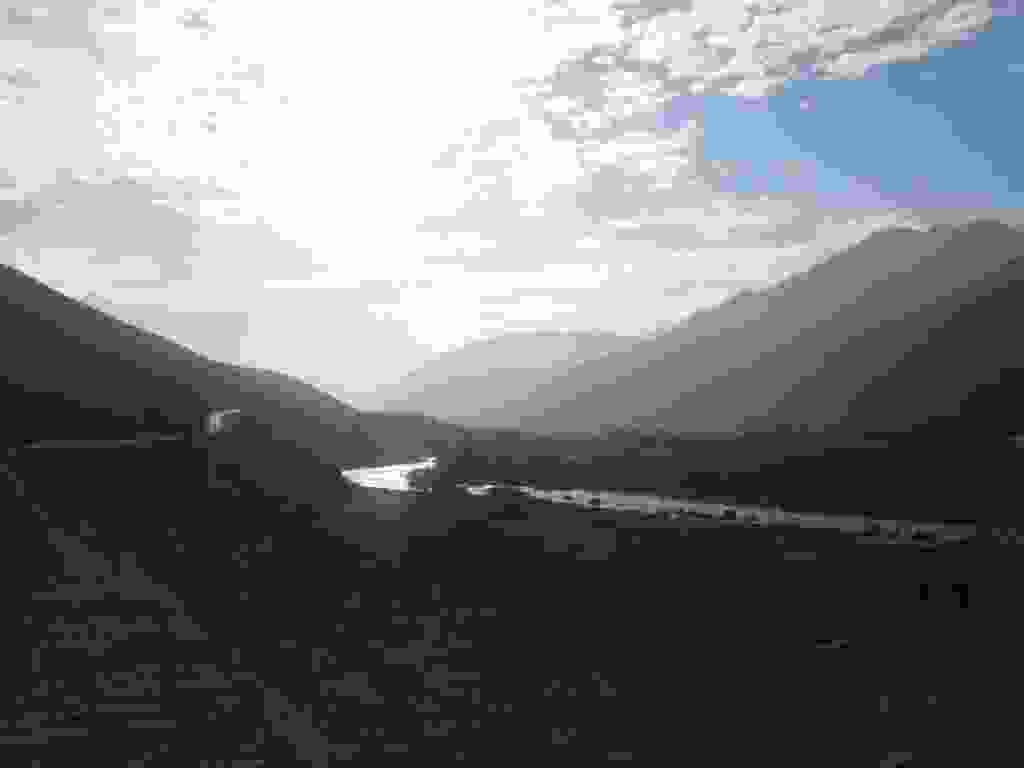
\includegraphics[height=90mm]{../wp-content/uploads/2015/06/P6094794-1024x768.jpg} } 
 \newline
 J´arrive dans le désert quasiment au niveau de la mer. La chaleur est étouffante surtout avec la poussière de la piste. \newline
 \newline
\centerline{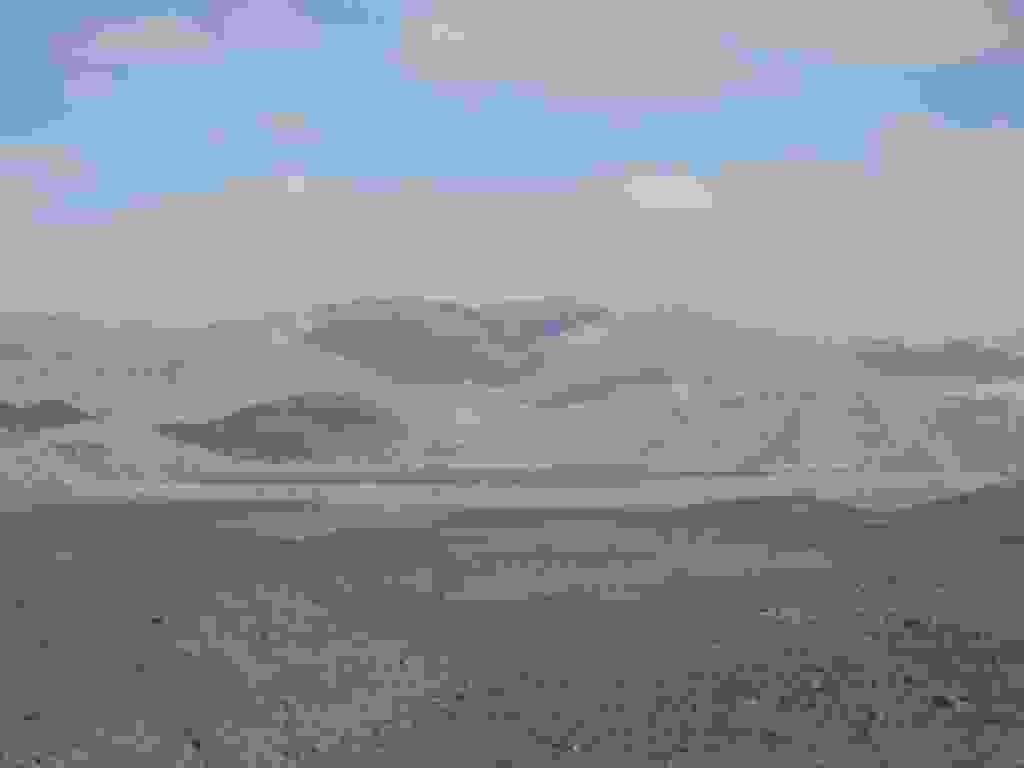
\includegraphics[height=90mm]{../wp-content/uploads/2015/06/P6094797-1024x768.jpg} } 
 \newline
 La dernière partie est sur la route panaméricaine. \newline
 \newline
\centerline{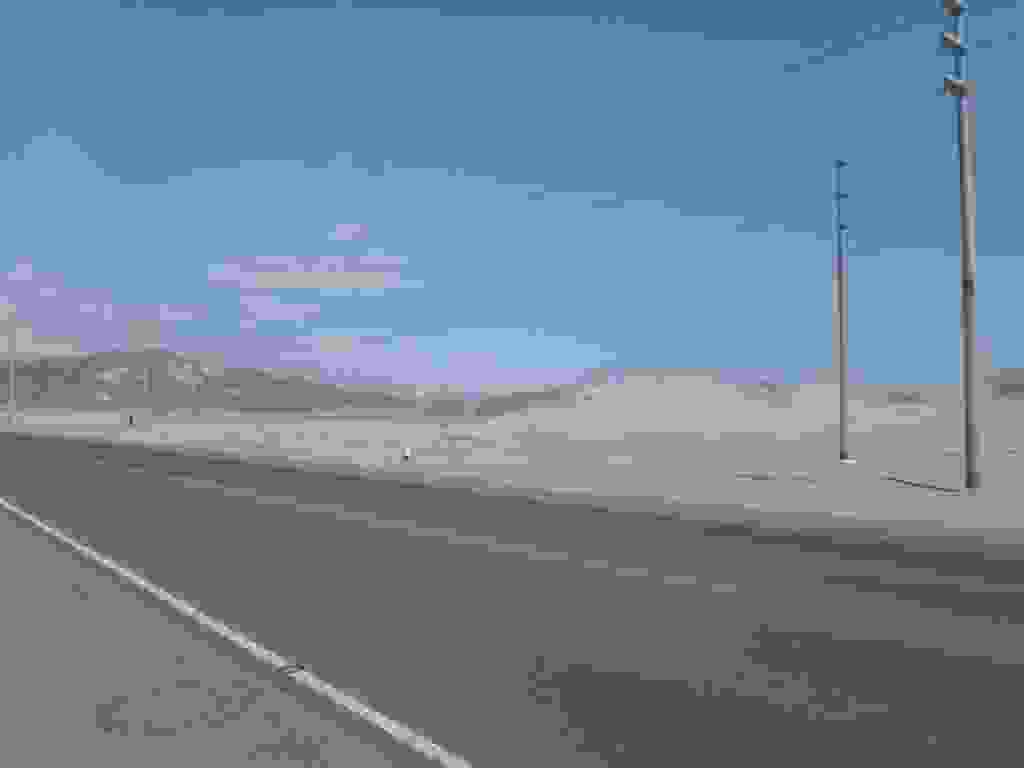
\includegraphics[height=90mm]{../wp-content/uploads/2015/06/P6094799-1024x768.jpg} } 
 \newline
 Enfin, j'arrive à Trujillo où je retrouve une casa de ciclistas, la plus ancienne d'Amérique du Sud tenue par Lucho. Je rencontre 3 cyclistes français, 2 belges et un américain. \newline
 \newline
\centerline{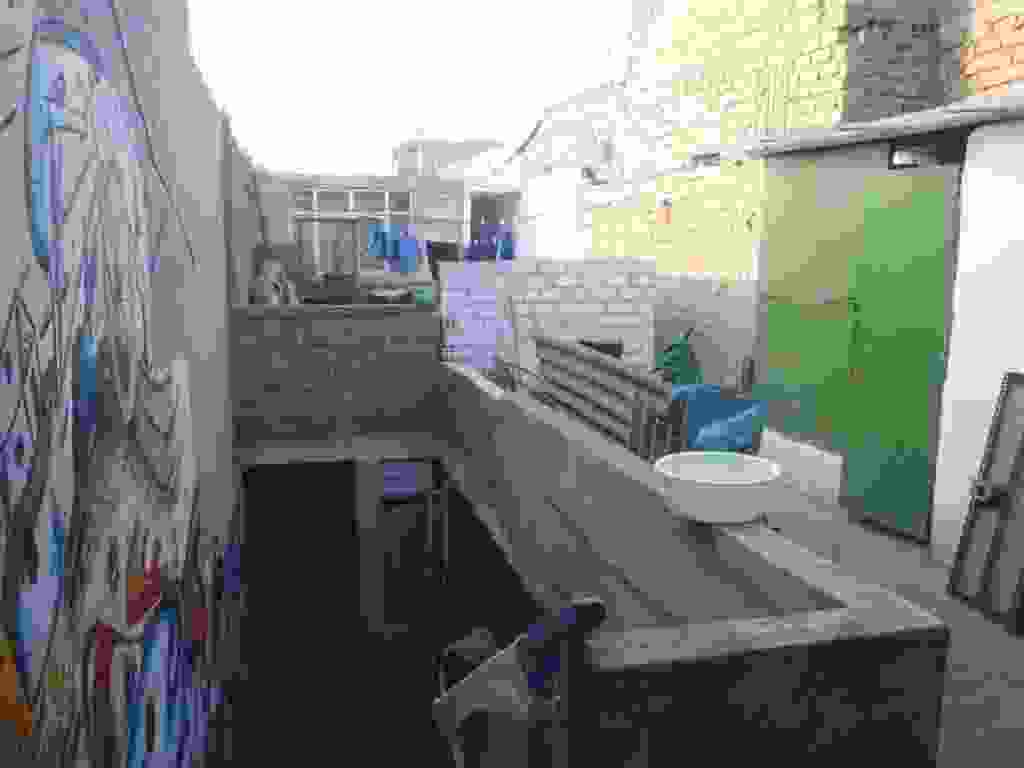
\includegraphics[height=90mm]{../wp-content/uploads/2015/06/P6114835-1024x768.jpg} } 
 \newline
 \newline
\centerline{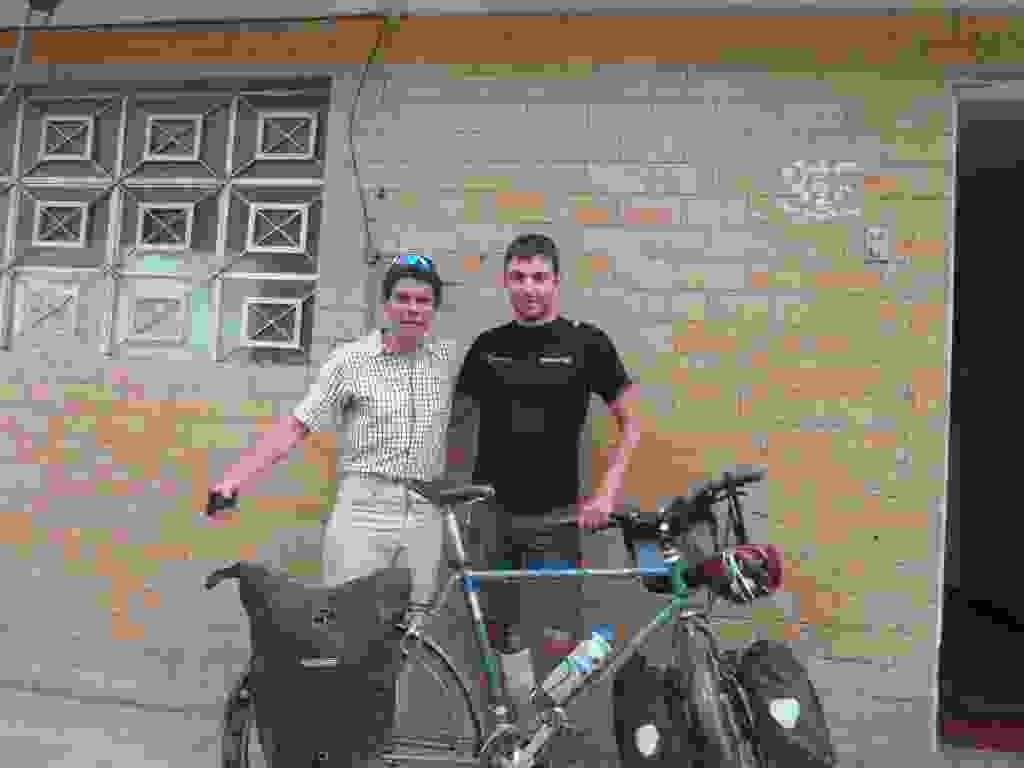
\includegraphics[height=90mm]{../wp-content/uploads/2015/06/P6114838-1024x768.jpg} } 
 \newline
 La place d´armes de Trujillo. \newline
 \newline
\centerline{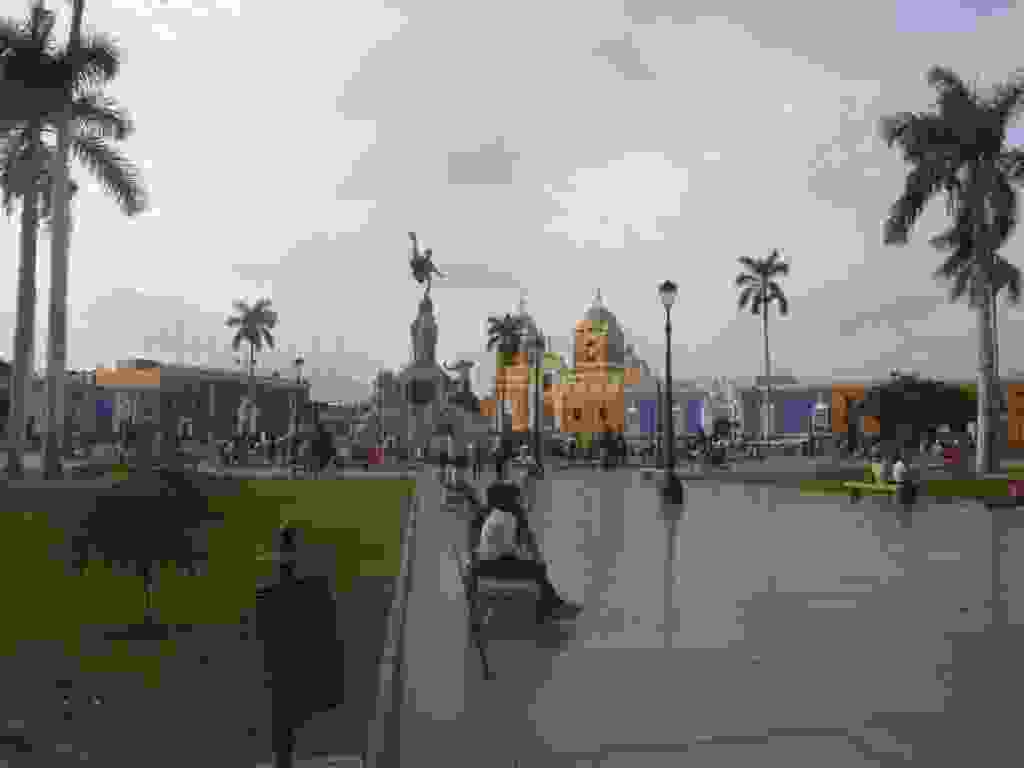
\includegraphics[height=90mm]{../wp-content/uploads/2015/06/P6104806-1024x768.jpg} } 
 \newline
 Les ruines de Chan Chan à quelques km, une cité pré inca construite tout en terre. \newline
 \newline
\centerline{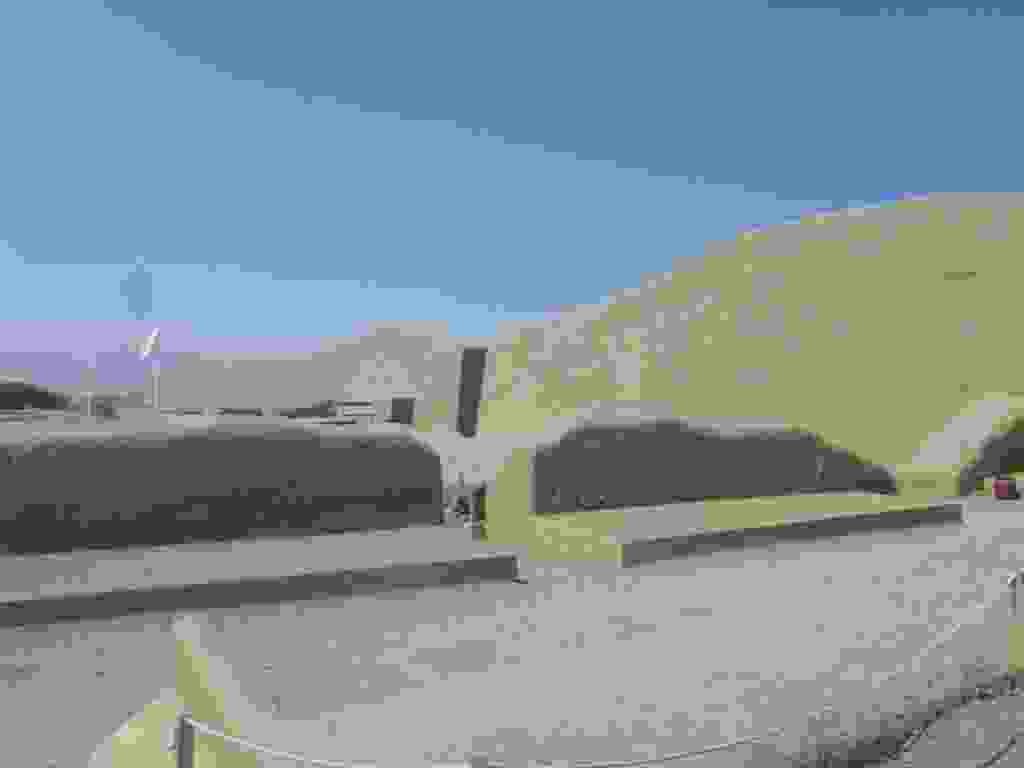
\includegraphics[height=90mm]{../wp-content/uploads/2015/06/P6104824-1024x768.jpg} } 
 \newline
 \newline
\centerline{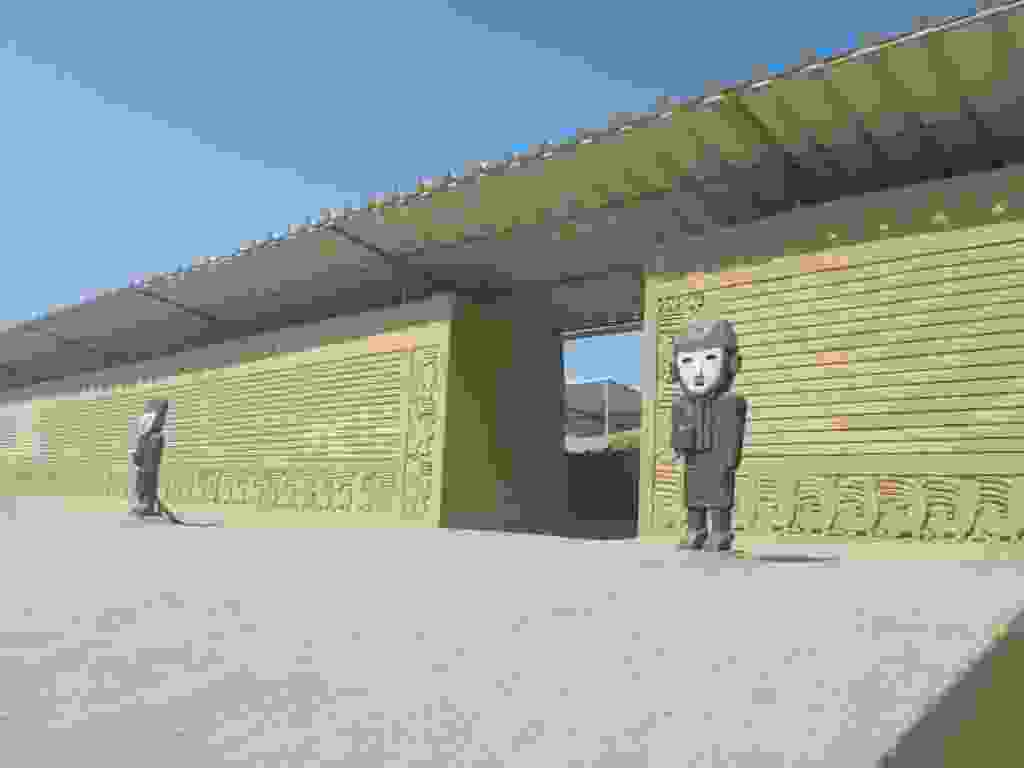
\includegraphics[height=90mm]{../wp-content/uploads/2015/06/P6104808-1024x768.jpg} } 
 \newline
 \newline
\centerline{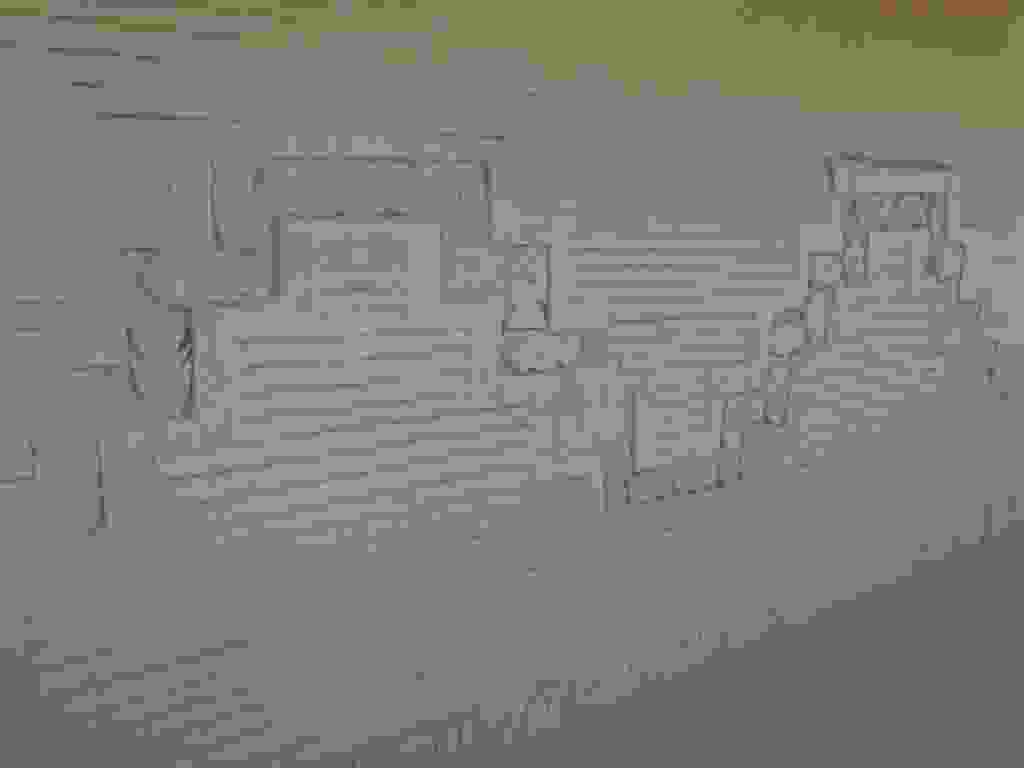
\includegraphics[height=90mm]{../wp-content/uploads/2015/06/P6104810-1024x768.jpg} } 
 \newline
 \newline
\centerline{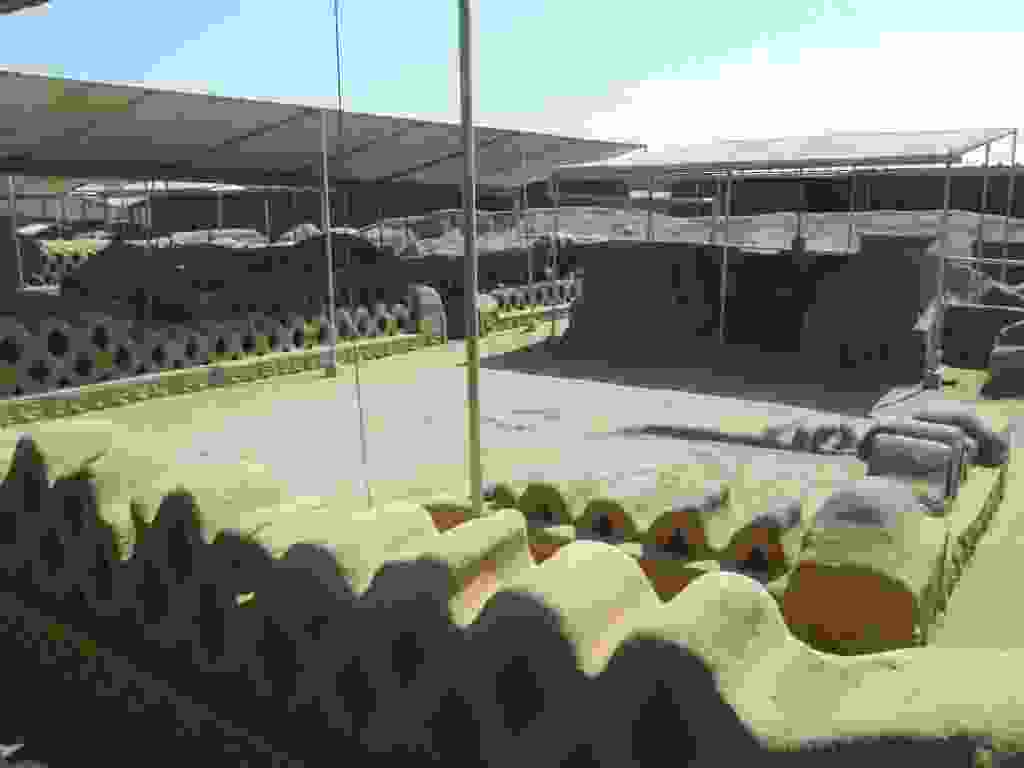
\includegraphics[height=90mm]{../wp-content/uploads/2015/06/P6104815-1024x768.jpg} } 
 \newline
 La station balnéaire de Huanchaco au bord du Pacifique : beaucoup de surfeurs et des pecheurs sur leurs embarcations en roseau. J'y ai croisé par hasard Jan avec qui j'avais fait le trek du Salkantay. \newline
 \newline
\centerline{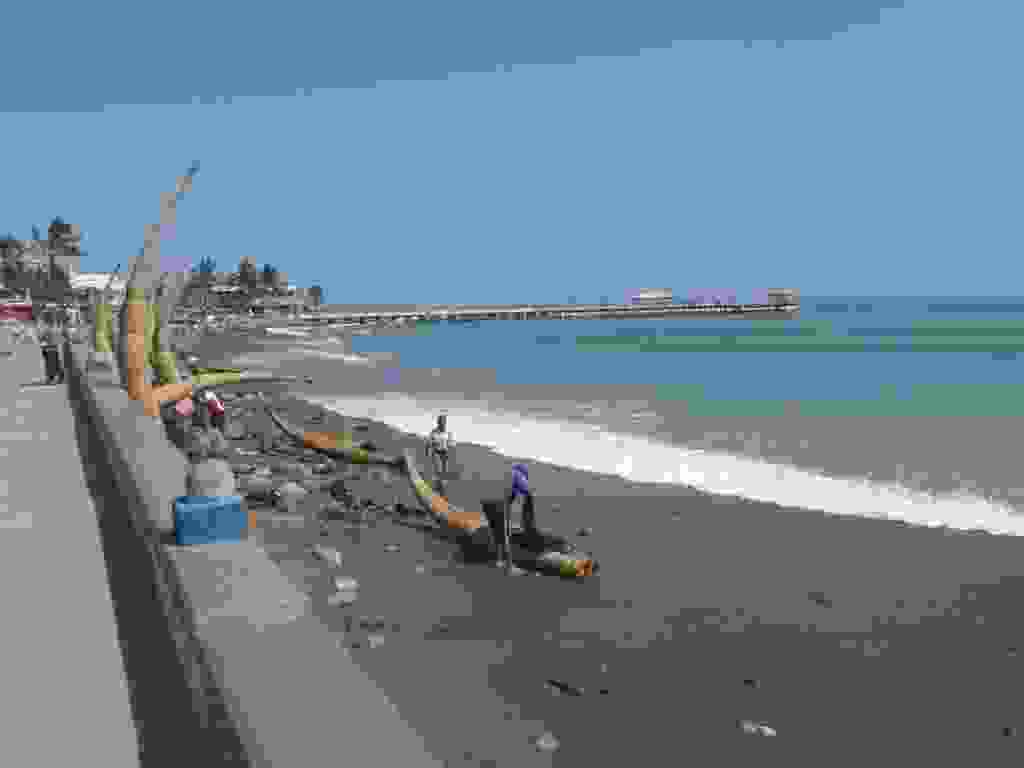
\includegraphics[height=90mm]{../wp-content/uploads/2015/06/P6104830-1024x768.jpg} } 
 \newline
 \newline
\centerline{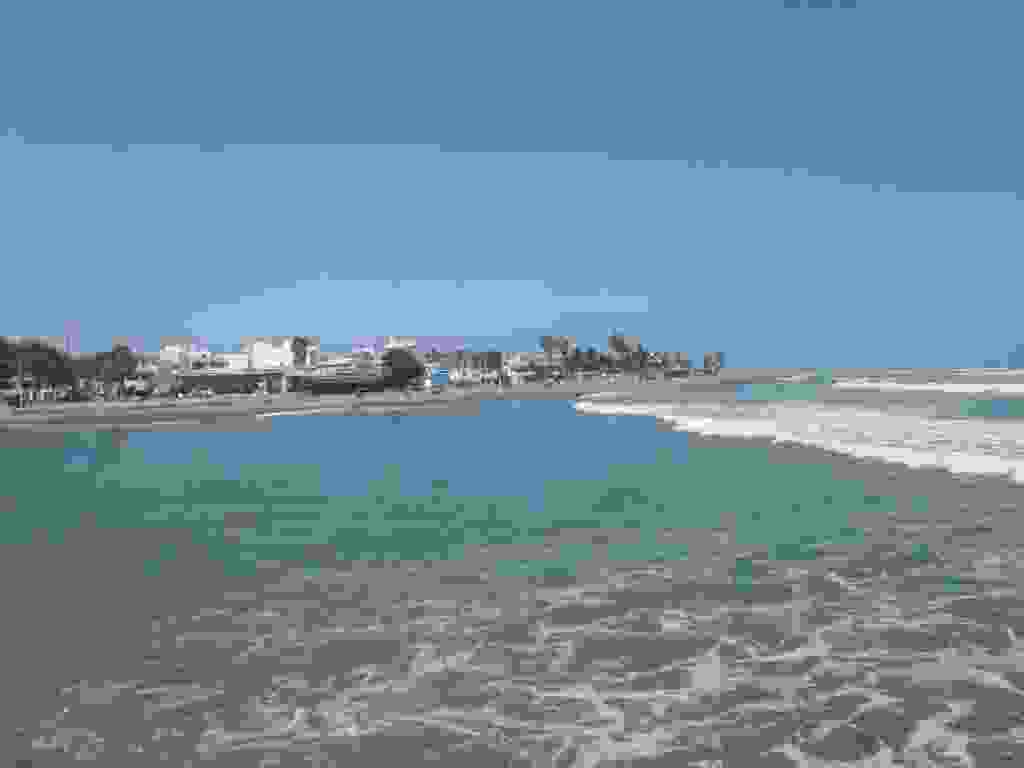
\includegraphics[height=90mm]{../wp-content/uploads/2015/06/P6104827-1024x768.jpg} } 
 \newline
 A bientot en Equateur ! \newline

\newpage
 
